% \nonstopmode
%%%%%
%%
%% Chalmers University of Technology Master's Thesis Template
%%
%% Jonas Einarsson (2010)
%% Adapted from work by Joel Goop
%%
%% Uses references.bib as Bibtex source
%% Uses elsevier numerical style .bst (change in settings.tex)
%%
%% DON'T FORGET: Change PDF metadata in settings.tex !!
%%
%%%%%
\documentclass[11pt,a4paper]{report}

% Packages and commands file
\usepackage[utf8]{inputenc}
\usepackage[T1]{fontenc}
\usepackage[swedish, english]{babel}
\usepackage{amsmath}
\usepackage{ae}
\usepackage{icomma}
\usepackage{units}
\usepackage{color}
\usepackage{graphicx}
\usepackage{epstopdf}
\usepackage{bbm}
\usepackage{caption}
\usepackage{multirow}
\usepackage{array}
\usepackage{geometry}
\usepackage{fancyhdr}
\usepackage{fncychap}
\usepackage[hyphens]{url}
\usepackage[breaklinks,pdfpagelabels=false]{hyperref}
\usepackage{lettrine}
\usepackage{eso-pic}
\usepackage{subcaption}
\usepackage[dvipsnames]{xcolor}
\usepackage{listings}
\usepackage[parfill]{parskip}
\lstloadlanguages{Ruby}
\lstset{%
basicstyle=\ttfamily\color{black},
commentstyle = \ttfamily\color{red},
keywordstyle=\ttfamily\color{blue},
stringstyle=\color{orange}}

\usepackage{fancyvrb}
\DefineShortVerb{\|}

\newcommand{\rd}{\ensuremath{\mathrm{d}}}
\newcommand{\id}{\ensuremath{\,\rd}}
\newcommand{\degC}{\ensuremath{\,\unit{^\circ C}}}

% Fancyheader shortcuts
\newcommand{\setdefaulthdr}{%
%\fancyhead[L]{\slshape \rightmark}%
%\fancyhead[R]{\slshape \leftmark}%
\fancyfoot[C]{\thepage}%
}
\newcommand{\setspecialhdr}{%
%\fancyhead[L]{ }%
%\fancyhead[R]{\slshape \leftmark}%
\fancyfoot[C]{\thepage}%
}

\newcommand{\mail}[1]{\href{mailto:#1}{\nolinkurl{#1}}}
\newcommand{\backgroundpic}[3]{%
	\put(#1,#2){
		\parbox[b][\paperheight]{\paperwidth}{%
			\centering
			\includegraphics[width=\paperwidth,height=\paperheight,keepaspectratio]{#3}
			\vfill
}}}





% Settings (Metadata)
% References, choose bst-file
\bibliographystyle{elsart-num}

% PDF Metadata and link styles
\hypersetup{
		pdftitle={Master's Thesis: },%
		pdfauthor={Jonas Einarsson},%
    colorlinks=true,%
    citecolor=black,%
    filecolor=black,%
    linkcolor=black,%
    urlcolor=black
}

% Dropping initial letter color
\renewcommand{\LettrineFontHook}{\color[gray]{0.5}}

% Chapter headings style (fncychap)
\makeatletter
\ChNumVar{} % sets the style for digit
\ChTitleVar{\Huge\bfseries\centering} % sets the style for title
\ChRuleWidth{4pt} % Set RW=4pt
\ChNameUpperCase % Make name uppercase
\renewcommand{\DOCH}{
\centering
{\CNoV {\fontsize{60pt}{20pt}\selectfont\thechapter} }
\vskip 40\p@}
\renewcommand{\DOTI}[1]{%
\CTV\FmTi{#1}\par\nobreak
\vskip 40\p@}
\renewcommand{\DOTIS}[1]{%
\CTV\FmTi{#1}\par\nobreak
\vskip 40\p@}
\makeatother

% Single page abstract
\renewenvironment{abstract}%
{\begin{center} \bfseries \abstractname \end{center}}%
{\vspace{2\baselineskip}}%

% Figure & Table captions
\captionsetup{margin=10pt,font=small,labelfont=bf}
\captionsetup[table]{position=top}
\setlength{\extrarowheight}{4pt}
\addtolength{\headheight}{\baselineskip}

% Fancyheader (see packagescommands.tex for default/special)
\pagestyle{fancy}
\setdefaulthdr

% Stolen settings (unknown origin):
% Alter some LaTeX defaults for better treatment of figures:
% See p.105 of "TeX Unbound" for suggested values.
% See pp. 199-200 of Lamport's "LaTeX" book for details.
%   General parameters, for ALL pages:
\renewcommand{\topfraction}{0.9}	% max fraction of floats at top
\renewcommand{\bottomfraction}{0.8}	% max fraction of floats at bottom
%   Parameters for TEXT pages (not float pages):
\setcounter{topnumber}{2}
\setcounter{bottomnumber}{2}
\setcounter{totalnumber}{4}     % 2 may work better
\setcounter{dbltopnumber}{2}    % for 2-column pages
\renewcommand{\dbltopfraction}{0.9}	% fit big float above 2-col. text
\renewcommand{\textfraction}{0.07}	% allow minimal text w. figs
%   Parameters for FLOAT pages (not text pages):
\renewcommand{\floatpagefraction}{0.7}	% require fuller float pages
% N.B.: floatpagefraction MUST be less than topfraction !!
\renewcommand{\dblfloatpagefraction}{0.7}	% require fuller float pages

% remember to use [htp] or [htpb] for placement


\usepackage[parfill]{parskip}
\usepackage{amsthm}

\begin{document}

% Title page and abstract
% Chalmers title page
\begin{titlepage}

\AddToShipoutPicture{\backgroundpic{-4}{56.7}{fig/auxiliary/frontpage}}
\mbox{}
\vfill
\addtolength{\voffset}{2cm}
\begin{flushleft}
	{\noindent {\Huge Water} \\[0.5cm]
	\emph{\Large En ersättning för Fire, baserad på versionshantering} \\[2.8cm]
	
	{\huge JESPER JOSEFSSON    }\\[.8cm]
	{\huge SOFIA LARSSON       }\\[.8cm]
	{\huge LINUS OLEANDER      }\\[.8cm]
	{\huge ARASH ROUHANI-KALLEH}\\[.8cm]
	{\huge PONTUS SAHLBERG     }\\[.8cm]
	{\huge JONAS ÄNGESLEVÄ     }\\[.8cm]
	
	{\Large Department of Computer Science \& Engineering \\
	\textsc{Chalmers University of Technology} \\
	Gothenburg, Sweden 2012 \\
	Bachelor's Thesis 2012:11\\
	} 
	}

\end{flushleft}

\end{titlepage}
\ClearShipoutPicture
% End Chalmers title page

\pagestyle{empty}
\newpage
\clearpage
\mbox{}
\newpage
\clearpage
\thispagestyle{empty}

\begin{abstract}
    Syftet med projektet som rapporten beskriver är att utveckla ett inlämningssystem för laborationer. Systemet ska bygga på versionshantering och ska hantera inlämning via en terminalklient. Inlämning skall även vara möjlig via ett webbgränssnitt.

    Systemets kärna är en webbapplikation som är baserad på open source-plattformen Gitorious, som är implementerad i Ruby on Rails. Systemet har en avancerad webbklient som flitigt nyttjar MVC-strukturerade Javascript-applikationer. Processintensiva arbeten delegeras till ett system av prioritetsköer och workers. WebSocket-protokollet används för asynkron kommunikation mellan webbservern och klienten. 

    Systemet använder sig utav BDD-ramverket RSpec för att få en självdokumenterande, högkvalitativ kodbas.

    Projektets omfattning visade sig vara för stort för tidsrymden av ett kandidatarbete, men resulterade i en mogen backend och ett välutvecklat gränssnitt som hanterar inlämning samt rättning av inlämningsuppgifter.

\end{abstract}
\selectlanguage{english}
  \begin{abstract}
    The purpose of the project described in the report is to develop a system for receiving and processing hand-in assignments. The system should be based on a version control system. The system should be able to receive hand-ins via a version control system command line client. Hand-in should also be possible via a web interface.

    A web application based on the open source platform Gitorious and Ruby on Rails is used to implement the system. The system features an advanced web client which makes extensive use of Javascript applications structured using the MVC design pattern. Process-intensive jobs are referred to a system of priority queues and workers. The WebSocket protocol is used for asynchronous communication between the web server and the client.

    The system uses the BDD-type test framework Rspec in order to make the code base self-documenting and to ensure high quality code.

    The scope of the project was found to be too wide, but the result was a mature backend and a well developed frontend for handing in and reviewing assignments.
  \end{abstract}
\selectlanguage{swedish}



% Table of contents
\newpage
\pagenumbering{roman}
\setcounter{page}{1}
%\pagestyle{fancy}
%\fancyhead[LO,RE]{\slshape \leftmark}

%\fancyhead{}
%\fancyfoot{}
%\fancyhead[CO,CE]{---Draft---}

%\fancyhead[CO,CE]{---Draft---}

%\fancyfoot[C]{Confidential}

%\fancyfoot[RO, LE] {\thepage}

\setspecialhdr
\tableofcontents

% Main area
\newpage
\setdefaulthdr
\pagenumbering{arabic}	
\setcounter{page}{1}

% Content
\chapter{Inledning}

\section{Bakgrund}

\subsection{Inlämningsuppgiftens roll i datavetenskapliga utbildningar}

Inom datavetenskapliga utbildningar är inlämningsuppgifter, ibland kallade laborationer, ett vanligt pedagogiskt verktyg. I regel ställs studenterna inför någon form av problem som de ska lösa genom att programmera. Genom laborationerna får studenterna möjlighet att applicera koncept som tagits upp under föreläsningar och de kan ställas inför praktiska problem som inte berörs av undervisningen i övrigt. 

Antalet studenter på datavetenskapliga kurser kan vara stort vilket gör att den givande institutionen ställs inför ett praktiskt problem – hur hanterar man inlämning och rättning av en stor mängd inlämningsuppgifter på ett effektivt sätt?

Svaret är ett specialiserat system.

\subsection{Nuvarande system vid Chalmers tekniska högskola}

På Chalmers tekniska högskola används ofta Fire, ett webbaserat system som endast hanterar inlämning och rättning av inlämningsuppgifter.
Studenten skapar en användare och ansluter sig sedan till en grupp i Fires webbgränssnitt. Därefter väljer studenten en laboration att ladda upp filer till. När samtliga filer är uppladdade kan studenten välja att lämna in sina filer. 

Handledarna som rättar uppgifterna erbjuds ett gränssnitt för rättning. Administratören kan skapa kurser och delegera rättigheter, som att förändra deadlines, till handledare. Systemet erbjuder dessutom smidig hantering av kurser med studenter från olika universitet

Fire uppfyller grundförutsättningarna för ett fungerande system och har många uppskattade egenskaper.
Däremot finns det ett antal områden med utrymme för förbättring. Bland annat startar Fire en separat webbserverinstans för varje kurs. Detta leder till vattentäta skott mellan kurser. Studenter är tvungna att registrera sig på nytt för varje ny kurs och länken till webbgränssnittet är olika för varje kurs. Tidigare har antalet webbserverinstanser dessutom begränsats till 64. I nuläget har har denna artificiella gräns höjts, men i längden är det inte praktiskt att skapa en serverinstans per kurs.


Ett annat problem med Fire är att många operationer inte går att ångra eller ändra i ett senare skede. 
I Fire utnyttjas inte heller möjligheten att erbjuda mervärde till användarna. Kommunikationen mellan handledare och studenter är rudimentär – handledarens svar laddas upp via ett webbformulär och studenterna kan bara svara med en ny inlämning. Projektarbeten hämmas av att inlämning av större mängder filer eller mappstrukturer endast är möjligt med tar.gz-arkiv, (Gedell, T. Upload File. 2006 ).

Orsaken till att många problem kvarstår är att Fire saknar dokumentation på kodbasen och databasen. Detta gör det väldigt svårt att vidareutveckla Fire.
Det finns med andra ord mycket som talar för en helt ny lösning för inlämning och hantering av laborationer.

\subsection{Versionshantering}

Versionshantering är ett oumbärligt verktyg för programmerare. Konceptet \emph{branches} gör det lätt att utveckla nya funktioner utan att förstöra nuvarande kodbas. Versionshantering förenklar även arbetet i grupp genom att  stödja sammanslagning - merge - av olika grenar. Detta uppmuntrar till strukturerade arbetssätt, och effektivt samarbete. 

Backup och historik förflyttas från filnivå till funktionsnivå genom att man gör regelbundna commits. Dessa upptar dessutom nästan ingen plats eftersom systemen i regel inte sparar hela projektets tillstånd i en commit, utan bara skillnaden till föregående commit – så kallad $\Delta$-data.

I en commit förväntas programmeraren bifoga ett meddelande som beskriver ändringarna som har gjorts. Detta uppmanar fram en form av loggskrivande under utvecklingsprocessen.

Versionshantering underlättar även vid bugghantering, eftersom flera kända buggfria tillstånd ofta finns att hitta i historiken.

I projektgruppen använder vi redan versionhantering för att hantera våra inlämningsuppgifter.

Om ett inlämningssystem utformas så att det bygger på versionshantering skulle systemet kunna erbjuda inlämningar direkt från versionshanteringsklienten. Systemet skulle dessutom kunna utnyttja fördelarna med versionhantering, som att snabbt kunna visa skillnader mellan olika tillstånd i kodbasen.

\subsection{Syfte}

Huvudsyftet med projektet är att konstruera ett system med webbgränssnitt och
backend som hanterar inlämning och rättning av inlämningsuppgifter. Systemet ska
vara baserat på versionshantering.

\subsection{Centrala problemområden och frågeställningar}

Inlämning ska kunna ske direkt från ett system för versionshantering. För att fånga upp alla typer av användare ska inlämning även kunna ske via andra kanaler, till exempel via webbgränssnittet.

Systemet ska utformas så att det ger alla kategorier av användare en bättre användarupplevelse än tidigare system i kategorin, och då i synnerhet i jämförelse med Fire.

Studenter ska ges möjlighet till tät kommunikation med handledaren.

Inom projektets ramar ska frågor kring anonym rättning, statistik och plagiatkontroll undersökas.

Projektet ska undersöka möjligheterna att effektivisera inrapportering av resultat till LADOK.

Systemet ska erbjuda handledare eller examinator möjlighet att definiera tekniska och formella specifikationer för en inlämning som kan kontrolleras automatiskt. Inom projektets ramar ska möjligheten till avancerade automatiserade tester undersökas.

Systemet ska vara enkelt att underhålla och vidareutveckla.

\subsection{Disposition}

Rapporten följer gängse struktur: bakgrund, syfte, problemanalys, metod och design, diskussion och slutsats. För att hjälpa läsaren följa med i de många beslutsprocesserna – beslut som dessutom i många fall beror på varandra – så har vi valt att lägga in korta beslutsavsnitt efter vissa  problembeskrivningar och analyser. I avsnitten beskrivs besluten och deras motivering kort. För utförligare information om beslut hänvisar författarna till metod- och designavsnitten.
I många sammanhang nämns olika produkter och teknologier som kandidatgruppen har använt under analys eller utveckling av systemet. Dessa samlas tillsammans med sina respektive hemsidor i avsnitt \ref{sec:ordlista}.
\subsection{Ordlista}
\label{sec:ordlista}
\small
\begin{tabular} { | l | p{10cm} | }
\hline
\bf{Ord} & \bf{Betydelse} \\
\hline
Acceptance test	& Test som kontrollerar om koden uppfyller specifikationerna \\
\hline
Bare git-repositorium & En git-repositorium utav ett aktivt träd (working tree) \\
\hline
Blob & Binary large object \\
\hline
Branch & En gren i ett repositorium. \\
\hline
CommitRequest & Ett anrop som används av webbgränssnittet för att manipulera Git-repositorier \\
\hline
Constraint & Begränsning i databasen som bara tillåter data som följer en viss specifikation \\
\hline
Databas-agnostisk & Databas-agnostisk innebär att den fungerar med alla databaser \\
\hline
Databas-lager & Logik som implementeras i databasen ligger i databas-lagret \\
\hline
Databas-schema & Databasstrukturen utan data \\
\hline
DBMS & Databashanterare likt MySQL \\
\hline
Diff & Skillnaden mellan två kodbasstycken \\
\hline
Flash-socket & Websocket-lösning för ActionScript \\
\hline
Foreign key & Ett fält i en databastabell som pekar på en annan tabell \\
\hline
Hash & En heltalsrepresentation av någon sorts data \\
\hline
Hashfunktion & En algoritm som översätter data till ett heltal \\
\hline
Hash Fragment & Delen av en URL som kommer efter \# \\
\hline
LHG & LabHasGroup. Entitet som används för att koppla laborationsgrupper till laborationer \\
\hline
Modell-lager & Logik som implementeras i modellerna ligger i modell-lagret \\
\hline
MVC & Model-View-Controller, ett designmönster \\
\hline
Normaliserad databas & En icke redundant databas som följer normaliseringsreglerna \\
\hline
Longpolling & En förfrågan till extern server. Har servern ingen data att svara med så "hängs" förfrågan. \\
\hline
\end{tabular}

\begin{tabular} { | l | p{10cm} | }
\hline
\bf{Ord} & \bf{Betydelse} \\
\hline
Polling & Att underrätta sig om förändringar i tillstånd genom att göra upprepade förfrågningar \\
\hline
Git push & Publicering av lokal git till extern eller lokal server \\
\hline
Remote url & Git-url till extern eller lokal git-server \\
\hline
Repositorium & Datastruktur som kan innehålla flera versioner av en kodbas sparad på disk \\
\hline
REST & Representational State Transfer \\
\hline
Route & Sökväg eller URL till en viss del av en webbapplikation \\
\hline
Scopa & En namnrymd som kan enkapsulera saker inuti sig \\
\hline
Symmetrisk SHA1-signering & Signering av data m.h.a SHA1-algoritmen och ett konstant salt \\
\hline
Telnet & Nätverksprotokoll för textbaserad kommunikation \\
\hline
Trigger & En databasrutin som kan köras före, efter eller istället för en operation på en tabell  \\
\hline
Unit test & Test som kollar om en del av koden är redo att användas \\
\hline
Workers & Trådar som utför jobb i bakgrunden \\
\hline
Working tree & Det filträdet man jobbar med \\
\hline
\end{tabular}
\normalsize

\subsection{Länkar till produkter och teknologier}
\small
\begin{tabular} { | l | l | }
\hline
\bf{Produkt/Teknologi} & \bf{Länk} \\
\hline
Backbone.js & http://backbonejs.org/ \\
\hline
Bazaar & http://bazaar.canonical.com/en/ \\
\hline
Beanstalkd & http://kr.github.com/beanstalkd/ \\
\hline
Bundler & http://gembundler.com/ \\
\hline
Capybara & https://github.com/jnicklas/capybara/ \\
\hline 
CoffeeScript & http://coffeescript.org/ \\
\hline
Facebook & http://www.facebook.com/ \\
\hline
Faye & http://faye.jcoglan.com/ \\
\hline
Fire & http://fire.cs.chalmers.se/ \\
\hline
Git & http://git-scm.com/ \\
\hline
Github Inc. & https://github.com/ \\
\hline
Gitorious & http://gitorious.org/ \\
\hline
Grack & https://github.com/schacon/grack \\
\hline
HAML & http://haml.info/ \\
\hline
jQuery & http://jquery.com/ \\
\hline
JUnit & http://www.junit.org/ \\
\hline
Launchpad & https://launchpad.net/ \\
\hline
LESS & http://lesscss.org/ \\
\hline
MiniTest & http://docs.seattlerb.org/minitest/ \\
\hline
MySQL & http://www.mysql.com/ \\
\hline
PostgreSQL & http://www.postgresql.org/ \\
\hline
Redis & http://redis.io/ \\
\hline
Resque & https://github.com/defunkt/resque \\
\hline
RSpec & http://rspec.info/ \\
\hline
Ruby & http://www.ruby-lang.org/ \\
\hline
Ruby on Rails & http://rubyonrails.org/ \\
\hline
RubyGems & http://rubygems.org/ \\
\hline
SASS & http://sass-lang.com/ \\
\hline
SecureFaye & https://github.com/oleander/secure\_faye \\
\hline
Stomp & https://rubygems.org/gems/stomp \\
\hline
TestUnit & http://test-unit.rubyforge.org/ \\
\hline
\end{tabular}
\normalsize

\chapter{Domän - problembeskrivning och analys}

\section{Inlämningskanaler}

Det nya systemet ska vara anpassat för användare med olika kunskapsnivåer. En konsekvens av detta är att inlämning via versionshanteringsklient inte kan vara det enda tillvägagångssättet. Studenter vid olika program och vid olika skeden av sin utbildning kan ha varierad eller ingen erfarenhet av versionhantering. Det är därför viktigt att erbjuda flera kanaler.

\subsection{Git}
Git som inlämningskanal behandlas i  [HÄNVISNING TILL AVSNITT].

\subsection{Webbgränssnitt}
Uppladdning genom webbgränssnitt är den lösning som används i Fire. Metoden är robust och bekant för de flesta. Projektgruppen anser dock att lösningen lider av ett antal begränsningar. Det enda sättet att ladda upp flera filer på samma gång är med arkivfiler i tar.gz-format (Gedell, T. (2006), Upload File). Detta är också det enda tillgängliga sättet att ladda upp mappstrukturer. Det går heller inte att bläddra i innehållet i filer eller tar.gz-arkiv, vilket leder till att studenter ofta känner sig tvungna att ladda ner en hel inlämning igen för att känna sig säkra på att innehållet är korrekt.

Water bör erbjuda ett mer flexibelt sätt att ladda upp filer. Uppladdning av flera filer på samma gång bör vara möjligt. Det bör också gå att skapa mappar och ladda upp filer till olika ställen i en mappstruktur. För att detta ska vara möjligt bör Water möjliggöra navigering i filstrukturer.

\subsection{E-post}
Ytterligare en potentiell metod för inlämning är via e-post. Studenter skulle då kunna skicka in inlämningar som bifogade filer. För att knyta en inlämning till en specifik uppgift inom en viss kurs så skulle systemet kunna generera unika identifikationskoder som studenten skickar med i mailet. Förslagsvis skulle man vid registrering för en kurs i systemet få ett mail per uppgift som innehåller all information som behövs för att kunna utföra laborationen. Studenten skulle då kunna lämna in till en specifik uppgift genom att svara på mailet som är knutet till den uppgiften.

Som vi såg det skulle logiken för mailinlämningar riskera att bli väldigt invecklad. Om syftet med att utöka antalet inlämningskanaler är att höja användarvänligheten, så finns det ingen anledning att lägga till en kanal där inlämningsförfarandet är onödigt komplicerat.

\begin{flushright}
  \textbf{Beslut}
  
  Inlämningskanalerna begränsas till versionshanterare och webbgränssnitt för att undvika komplexiteten i att implementera inlämning via e-post.
\end{flushright}


\section{Frågor gällande inlämning via versionshantering}\label{sec:fragor-git}
I systemet behövs lämpliga sätt att relatera koncept inom versionhantering till inlämningsuppgifter. Frågan kan delas upp i två delar: hur inlämningarna ska förvaras och hur inlämningen sker.

\subsection{Förvaring av inlämningsuppgifterna}
Vad gäller förvaringen ser kandidatgruppen två alternativ:

Antingen skapas ett nytt repositorium för varje grupp och inlämningsuppgift, eller så sparas gruppens samtliga inlämningsuppgifter i ett repositorium, men i olika grenar.

I skarpa projekt har varje delprojekt ett eget repositorium. Särskilt vanligt är detta för distribuerade versionhanteringssystem, eftersom de ofta inte erbjuder clone för bara delar av ett repositorium. Se till exempel Git (git-clone(1) Manual Page, 2012). Kandidatgruppen är av uppfattningen att \emph{branches} traditionellt uppfattas som olika versioner av samma kodbas. Detta stöder idén om att använda ett repositorium per inlämningsuppgift. Det leder även till separation mellan inlämningsuppgifter – misstag eller tekniska problem inom en inlämningsuppgift inte drabbar andra inlämningsuppgifter. Metoden öppnar även för att Water i framtiden erbjuder studenterna flera \emph{branches} att arbeta med, till exempel för att definiera delmoment i inlämningsuppgifter eller som ett kollaborationsverktyg.

En nackdel med separata repositorier är att det krävs en \emph{remote-url} per repositorium, och därmed per inlämningsuppgift. För varje inlämningsuppgift måste studenten hämta en \emph{remote-url} ifrån webbapplikationen och använda den för att konfigurera sin versionshanterare.

\subsection{Inlämning via versionshantering}
Vad gäller själva inlämningen finns ett antal tänkbara strategier.

En möjlighet är att låta varje commit utgöra en inlämning. Metoden är lätt att implementera, men tillåter inte att studenterna bygger upp en inlämning med hjälp av ett antal commits och bidrar heller inte till kollaborering.

En annan möjlighet är att använda taggar. Taggar är ett sätt att knyta metadata till ett visst tillstånd i versionshanteringsträdet. Taggar kräver dock ofta att användaren lär sig en speciell syntax. I Git, exempelvis, krävs dessutom att användaren uttryckligen begär att taggar ska skickas med när ändringar överförs via en push till en annan nod.

Ett alternativ till taggar är att definiera speciella strängar som användaren kan skriva in i commit-meddelandet. Versionshanterar-servern analyserar alla inkommande commits för att leta efter dessa. Denna metod används bland annat av code hosting-tjänsten Github för att göra det möjligt att knyta en commit till en issue i deras issuehanteringssystem. Där räcker det med att skriva \#1 för att referera till issue nummer 1. Water skulle kunna lyssna efter en lämplig sträng som signalerar att commiten i fråga ska utgöra en inlämning.

\begin{flushright}
  
  \textbf{Beslut}
  
  För varje inlämningsuppgift har en grupp ett repositorium. I systemet definieras en \emph{branch} som global inlämningsbranch. I vårt fall är det master som används för inlämningar. Inlämningar kan konstrueras som ett antal commits, själva inlämningen sker genom att commit-meddelanden innehåller strängen \#submit.
\end{flushright}

\section{Inlämningens livscykel}

Grundantagandet i Water är att en inlämning i sin enklaste form är en pekare till ett visst tillstånd i ett repositorium – en commit. Inlämningen går igenom ett antal tillstånd innan uppgiften kan godkännas. När denna livscykel ska utformas ställs krav som enkelhet, flexibilitet och tydlighet mot varandra.

\subsection{När ska inlämningskanalerna öppnas och stängas?}
Grundidén är att inlämningskanalerna stängs när deadline passerat eller när en inlämning har gjorts för att undvika att rättaren arbetar med en inlämning som inte längre är aktuell. Kanalerna öppnas igen om inlämningen är underkänd.

Ur studenternas perspektiv är det dock önskvärt att kunna göra ändringar i en inlämning så länge som möjligt. En typisk situation är att filer fattas eller att något uppenbart fel uppdagas efter att inlämning har skett. Det förefaller onödigt att låta studenterna vänta på att en rättare underkänner inlämningen innan de kan rätta felet.

En kompromiss är att tillåta ändringar i en inlämning tills rättaren har börjat arbeta med den. 

\subsection{Uppdatering av inlämningar}
Teoretiskt vore det möjligt att se ändringar av inlämningar som nya inlämningar. I så fall skulle studenterna ha rätt att göra ett obegränsat antal inlämningar tills dess att rättaren inleder sitt arbete. Detta leder dock till att det kan finnas föräldralösa inlämningar i systemet som aldrig kommer att behandlas, vilket gör hanteringen av dem svårare.

För att undvika detta är det möjligt att se ändringar i inlämningar som uppdatering av en befintlig inlämning. Vid uppdatering riktas pekaren i inlämningen till ett nytt tillstånd i inlämningsrepositoriet. Det öppnar även för enklare hantering av till exempel deadlines, eftersom till exempel den första deadlinen kan relateras direkt till den första inlämningen.

\subsection{När inlämningen har rättats}
Om en inlämning blir godkänd bör det inte längre vara möjligt att lämna in fler inlämningar. Om inlämningen däremot är icke-godkänd, och chans för ytterligare inlämning finns, bör inlämningskanalerna öppnas igen.

\begin{flushright}

  \textbf{Beslut}

  En inlämning kan uppdateras så att den pekar på ett nytt tillstånd i ett repositorium tills handledaren har börjat rätta den. Blir inlämningen underkänd kan en ny inlämning skapas. Blir inlämningen godkänd är det inte längre möjligt att lämna in.
\end{flushright}

\section{Tillståndshantering - vilken entitet är det som blir godkänd?}

För att implementera inlämningens livscykel behövs ett antal tillstånd och strategier för att hantera de olika stegen.

För betygssättning behövs tillstånd för godkända och underkända inlämningar. För att kunna implementera uppdatering av inlämningar, vilket behandlas i avsnitt \ref{sec:uppdatering-inlamningar}, behövs skilda tillstånd för inlämningar som väntar på bearbetning av handledare och inlämningar där arbetet har inletts.

Vid första anblick är det oklart vilken entitet i modellen som ska hantera dessa tillstånd. Tydligt är dock att handledarna i första hand kommer att behandla inlämningar för att kunna sätta ett betyg på en inlämningsuppgift. Den naiva lösningen är alltså att låta inlämningsentiteterna hantera tillstånd.

Det är på samma gång tydligt att det är grupper som får hela inlämningsuppgifter godkända, vilket talar för att tillståndet istället lagras i en entitet som kopplar grupper till uppgifter.

\subsection{Tillståndshantering i flera entiteter leder till redundans}
Ytterligare en lösning är att placera tillstånden där de tycks passa bäst – både i inlämningentiteten och i entiteten som kopplar grupper till laborationer. Detta skapar dock redundans i modellen eftersom informationen finns tillgänglig även om den bara sparas i den ena entiteten. Till exempel betyder en godkänd inlämning att även laborationen är godkänd. En godkänd laboration betyder att den sista inlämningen är godkänd och de övriga är icke-godkända eller icke rättade, beroende på hur modellen är beskaffad.

Redundans bör undvikas av de anledningar som diskuteras i kapitel \ref{sec:databasen}.

\subsection{Tillståndshantering i endast en entitet kan leda till oklara tillstånd}
Om tillståndshanteringen endast placeras i inlämningsentiteten blir det lätt att hämta information om enskilda inlämningar. Däremot måste alla inlämningsentiteter för en grupp och en inlämningsuppigft hämtas och kontrolleras när systemet ska beräkna hela inlämningsuppgiftens tillstånd.

Om tillståndshanteringen istället placeras i entiteten som kopplar grupper till inlämningsuppgifter är det lätt att hämta information om gruppens tillstånd i förhållande till inlämningsuppgiften. Det kan i gengäld bli svårare att ta reda på tillståndet för en enskild inlämning, beroende på hur modellen är uppbyggd. Problem uppstår om systemet tillåter föräldralösa inlämningar, vilket beskrivs i avsnitt \ref{sec:uppdatering-inlamningar}, och gruppen har gjort två eller flera inlämningar och den sista inlämningen är icke-godkänd. I detta fall är det omöjligt att veta om inlämningarna före den icke-godkända inlämningen är icke-godkända eller föräldralösa. Det går att betrakta alla inlämningar före en icke-godkänd inlämning som icke-godkända, men det leder till att inlämningar som aldrig har behandlats av en handledare ser ut att ha blivit behandlade.

Om systemet inte tillåter föräldralösa inlämningar går det att entydigt bestämma enskilda inlämningars tillstånd utifrån gruppens tillstånd i relation till inlämningsuppgiften.

\begin{flushright}

  \textbf{Beslut}

  Tillstånd hanteras i entiteten LabHasGroup, som beskrivs i modellavsnittet \ref{sec:modell-labhasgroup}. Entiteten representerar grupper i relation till inlämningsuppgifter. Enligt tidigare beslut tillåts inte föräldralösa inlämningar, vilket gör att enskilda inlämningars tillstånd kan entydigt bestämmas.
\end{flushright}

\section{Validering av inlämningar}\label{sec:valideringar}

I laborationer finns i allmänhet krav som måste uppfyllas för att de skall bli godkända. Typiska exempel på detta kan vara att inlämningen skall bestå av filer med speciella namn, ha en viss typ av filformat, maximalt antal tecken i radbredd eller gå igenom de tester som bifogats med laborationsbeskrivningen.

I det nuvarande systemet måste handledare manuellt neka inlämningar som inte uppfyller dessa krav. Handledarna får spendera tid på att avvisa laborationer som inte är giltiga då studenterna har slarvat med innehållet, men kanske har en korrekt lösning. Studenterna i sin tur förlorar ett av sina inlämningsförsök och blir först medvetna om detta efter att handledaren fått tid att titta på den.

En lösning till detta vore att i det nya systemet erbjuda automatiska valideringar vid varje inlämning. Dessa skulle kunna, så fort testerna är klara, meddela studenten om inlämningen uppfyller de grundläggande kraven - så denne får en omedelbar chans att rätta till felaktigheterna. Oftast har studenterna endast ett begränsat antal inlämningar på sig innan en laboration måste vara godkänd. Om en inlämning som inte passerar testerna skall minska antalet kvarvarande försök eller ej är något som skulle behövas ta ställning till.

Vad som skulle ingå i valideringen av en inlämning skulle behöva konfigureras efter specifikationerna för varje laboration. 

\begin{flushright}
  
  \textbf{Beslut}
  
  Möjlighet till valideringar undersöktes under projektet, men implementerades inte. Dock är funktionaliteten högprioriterad vid vidareutveckling av systemet.
  
\end{flushright}
\section{Rättning}

I Fire finns ett antal uppskattade funktioner för handledare. Bland annat kan handledaren ladda ner samtliga inlämningar som den ska rätta i ett tar.gz-arkiv (Gedell 2006b). Funktioner som dessa bör finnas även i Water.

Fire har dock några brister i rättningsfunktionen.

Handledare upplever ibland att det är svårt att se exakt vad som har ändrats mellan två inlämningar\footnote{Intervju med Oskar Utbult den 2 mars 2012}. Genom att som i Water basera inlämningssystemet på versionshantering är det lätt att ta fram skillnaden mellan två tillstånd – en såkallad \emph{diff}. En handledare som använder sig av ett versionshanteringssystem för att hämta inlämningar kan enkelt skapa en \emph{diff} själv. Water bör erbjuda visualisering av \emph{diffar} i webbgränssnittet.

Fire låter användaren hämta rena textfiler via webbgränssnittet, men kan inte hantera mappstrukturer. Studenter som vill lämna in projekt med annat än en endimensionell mappstruktur måste använda arkivfiler för att göra detta. Detta innebär även att handledarna måste ladda ner projekten som arkivfiler, istället för att förhandsgranska den i webgränssnittet.

Många inlämningar vore möjliga att rätta direkt i ett webbgränssnitt om det erbjöd navigering i mappstrukturer och rendering av källkodsfiler. Detta skulle göra handledarnas jobb mer flexibelt. Water bör erbjuda denna funktionalitet.

\begin{flushright}
  
  \textbf{Beslut}
  
  Water erbjuder uppladdning av flera filer på samma gång, bläddring i mappstrukturer, manipulation av mappstrukturer och rendering av källkod. Nedladdning av inlämningar i arkivformat och visning av diffar implementeras inte, men är högprioriterat vid vidareutveckling av systemet.
  
\end{flushright}
\section{Insyn i rättningsprocessen}

Från projektgruppens sida finns det en önskan om större insyn i rättningsprocessen.

En möjlighet är att upprätta ett kösystem. Samtliga inlämningar i hela kursen läggs i en rättningskö där de prioriteras efter vilken uppgift inlämningen gäller, inlämningstid, om inlämningen är svar på en retur och andra liknande faktorer. En ledig handledare skulle vara tvungen att rätta den inlämning som står längst fram i kön, i detta fall skulle studenterna få väldigt exakta uppgifter om sin köplats. Problemet med detta system är att reglerna för kösystemet skulle bli tämligen rigida och att de nödvändigtvis inte skulle passa för alla sorters kurser.

En annan möjlighet är att ge handledarna den information som de behöver för att själva göra prioriteringarna utan att bygga en tvingande kö i systemet. På detta sätt är systemet mer flexibelt men det skulle bli svårt att ge studenterna tydliga indikationer om hur rättningen fortskrider.

En kompromiss är att inlämningarna delas in i mindre prioritetsköer beroende på vilken laboration de hör till. Handledarna väljer vilken laboration de vill rätta, men är bundna till prioritetsköerna för den valda laborationen. 

\begin{flushright}

  \textbf{Beslut}

  Inga rigida prioritetsköer implementeras för rättning. Rättarna får göra prioriteringarna själva. Detta eftersom behoven i olika kurser kan variera på sätt som projektgruppen inte kan förutse.
\end{flushright}

\section{Anonym rättning}

På CTH har anonym rättning införts för alla salstentamina (Chalmers Studentportal, Anonyma tentor). För att förbättra studenternas rättssäkerhet valde kandidatgruppen att utreda om anonym rättning kunde införas även för laborationer.

Fördelar med anonym rättning är att studenter är garanterade en rättvis rättning där rättarens personliga åsikter inte kan påverka resultatet, anonym rättning innebär också att studenter kan argumentera med sina lärare om kursen och dess innehåll utan att oroa sig för negativa effekter vid bedömning.

Ett enkelt sätt att implementera detta på är att ersätta studenternas namn med sifferkoder eller liknande i vyerna. Då är det sparat i databasen vem det är och en administratör kan lämna ut uppgifterna om en elev eller grupp om nödvändigt.

Anonym rättning lämpar sig inte nödvändigtvis för alla sorters laborationer och så länge det inte finns något policybeslut om det från universitetet bör användandet av funktionen vara valbart för var kurs.

\begin{flushright}

  \textbf{Beslut}

  Då anonym rättning inte är en kritisk del av projektet har det blivit nedprioriterat.
Eftersom implementetationen är relativt enkel kommer den här funktionen troligtvis dyka upp i en senare version av mjukvaran.
\end{flushright}

\section{Kommunikation}

Ett syfte med Water är att förbättra kommunikationen mellan studenter och personal. Dessa förbättringar kan ske på olika nivåer.

Ett system som Water skulle kunna användas som allmän informationskanal, till exempel för meddelanden som handlar om kursval och dylikt,  eftersom det har tillgång till samtliga studenter som är registrerade på en kurs. Alla kurser på en institution kommer dock inte att använda Water. Därför är det bättre att använda andra verktyg för allmän kommunikation med studenterna. Fokus i Water ligger istället på att förbättra den kommunikation som sker mellan studenter och handledare i anknytning till inlämningsuppgifter.

\subsection{Kommunikation kring inlämningsuppgifter}
Som tidigare nämnt kan handledare i Fire inkludera kommentarer när de rättar en inlämningsuppgift. Studenterna kan endast svara med en ny inlämning. Studenterna riskerar att missuppfatta återkopplingen, vilket kan leda till att även den korrigerande inlämningen förkastas onödan. För att råda bot på detta vill projektgruppen att Water  ska erbjuda en dialog mellan handledare och student.

Detta kan implementeras genom ett kommentarssystem. Systemet låter handledare kommentera inlämningar. Handledarens kommentarer presenteras sedan tillsammans med koden i webbgränssnittet. Studenterna kan därefter svara på handledarens kommentarer med egna kommentarer.

Ytterligare en möjlighet är att erbjuda så kallade inline-kommentarer, det vill säga kommentarer som är knutna till specifika rader i inlämnade filer. Detta skulle göra det möjligt för handledarna att ge återkoppling på väldigt specifika problem, istället för att försöka referera till dem i löpande text i en kommentar till inlämningen.

Alla parter bör bli underrättade när nya kommentarer har kommit in.

\section{Laborationsgrupper i Water}

Fire möjliggör för studenter att arbeta i nya grupper under varje laboration. I systemet kan en student skapa flera grupper och bjuda in olika personer till var grupp. Vid kursslut förstår Fire huruvida en student avklarat alla laborationer i kursen oavsett i vilken av sina grupper laborationen fullgjorts. Vanligtvis laborerar elever i samma grupp under en  hel kurs men systemet behöver kunna hantera studenter som jobbar i olika grupper i samma kurs.

Laborationsgrupperna i Water kommer att efterlikna funktionaliteten som finns Fire och utvidga den.

\subsection{Avhopp från laborationsgrupper}
Av olika skäl kan det finnas behov av att splittra grupper.  Till exempel kan studenterna ha blivit oense eller avregistrerat sig från kursen. Konceptuellt måste det vara möjligt att dela upp grupper. Den naiva lösningen är att bara radera en grupp och att skapa nya. När en grupp raderas försvinner alla inlämningar den gruppen har gjort då det inte får finnas Git-repositorier som inte tillhör någojen grupp, detta leder också till att informationen som anger vilkaimalt laborationer gruppen har klarat raderas.

\begin{itemize}
  \item En student som avregistrerat sig från en grupp skall ej få godkänt på laborationer som kvarvarande i gruppen lämnar in.
  \item Ingen data skall tas bort vid avhopp, speciellt inte avklarade laborationer.
  \begin{itemize}
    \item Studenternas material måste finnas kvar och vara tillgängligt för dem.
  \end{itemize}
  \item Som en studentanvändare av Water vill man känna sig trygg med att splittringsoperationen inte tar bort något. Till exempel måste inskickade laborationer förbli inskickade och rättas för alla deltagare i den splittrade gruppen. Den splittrade gruppen bör kunna fortsätta arbeta tillsammans vid retur, även om de börjat arbeta i nya grupper. En student skall alltså kunna förstå med hjälp av gränssnittet att ovanstående situation gäller när de splittrar gruppen.
\end{itemize}

Vi presenterar nedan två lösningsideer som gruppen övervägde mellan. I lösningarna tar vi upp perspektiv både på användargränssnitt och databasmodell.

\subsection{Faktisk splittring av grupper}
Ett naturligt sätt att utföra splittringen på är att försöka efterlikna det konceptuella att en eller flera studenter faktiskt hamnar i en ny grupp medan resterande är kvar. För att de nya studenterna ska kunna ha kvar sitt material från sin splittrade grupp krävs det att de avklarade laborationerna kopieras över till deras nyskapade grupp. Att kopiera data i en databas anses som allmänt fel då en \emph{normaliserad} databas, vilket beskrivs djupare i kapitel \ref{sec:databasen}, ska ha minimalt med redundans. Man kan också låta laborationer “ägas” av själva studenterna och inte gruppen. I detta fall kommer en splittrad grupp inte påverka studenternas datatillgång eftersom den inte baseras på grupper.

\subsection{Immuterbara grupper}
En annan lösning är att låsa medlemmarna i en laborationsgrupp, vilket innebär att man inte kan splittra en grupp. Paradigmen blir då att gruppen motsvarar en fixt grupp av studenter. Att på detta sätt ha oföränderliga grupper löser direkt problemet med hur man kopierar över material till nya grupper, eftersom grupper aldrig splittras. Operationen av en konceptuell splittring för en grupp på två studenter kommer utföras genom att båda studenter skapar var sin ny grupp, alternativt går med i redan existerande grupper. Ett till problem som löses med detta är att studenter inte heller kan gå med i en låst grupp, alltså en student som inte utfört en laboration kan inte bara gå med och få godkänt på tidigare laborationer avklarade av den gruppen.

Också denna lösning introducerar problem, nämligen att definiera hur en grupp bildas och populeras med studenter. Om alla grupper börjar frysta skulle en nyskapad grupp förbli tom.

Det är inte självklart att immuterbara grupper är begripligt för en studentanvändare.  Vi vet inte om en grupp elever som vill splittras naturligt tänker sig att de “splittrar” sin grupp eller om de direkt förenklar det till att de skapar varsin ny grupp.

\begin{flushright}

  \textbf{Beslut}

  Vi valde immuterbara grupper för det är enklare då vi egentligen inte behöver implementera splittring av grupper. Immuterbarheten möjliggör även att forcera invarianter för studenters laborationsantal.
\end{flushright}

\section{Invarianter för studenters laborationsantal}

Det finns möjlighet att ha en invariant mellan hur många simultana “laboration-till-grupp”-kopplingar det finns per laboration för varje enskild student. Det rör sig mellan alternativen att forcera maximalt en koppling per laboration, att forcera till exakt en koppling per laboration samt att strunta i att ha invarianten. Det leder till mer arbete att uppehålla en striktare invariant, men det har fler fördelar.

För att göra detta avsnitt läsbart inför vi termen LabHasGroup, förkortad LHG. LHG är den entitet i modellen som representerar kopplingen mellan en grupp och en laboration. [HÄNVISA TILL MODELL-KAPITEL]

\subsection{Max en LHG per laboration ($\leq 1$)}
Som en direkt konsekvens av denna invariant kan inte en student lämna in samma laboration genom flera laboration till grupp kopplingar eftersom invarianten direkt stryper kopplingsantalet till maximalt en per laboration. I praktiken jobbar aldrig en student på samma laboration via flera kopplingar samtidigt. Det är troligt att studentanvändare blir förvirrade av att de ser att de jobbar på samma laboration via olika kopplingar. Det bör alltså noteras att fördelarna är främst  ytliga, alltså att produktens webbinterface blir tydligt för studentanvändarna. Vidare ska en handledare inte av misstag behöva rätta två inlämnade laborationer kopplade till samma student.

Flera möjliga sätt finns för att enforcera invarianten, gemensamt för implementeringssätten är att de måste definera nödvändiga gruppoperationer och visa att de är riskfria, det vill säga att invarianten aldrig bryts efter operationerna har utförts. Några operationer kan tänkas vara följande:

\begin{itemize}
  \item Skapa grupp
  \item Gå med i grupp
  \item Eventuellt “starta laboration”
  \item Ta bort,  inaktivera eller frysa en laboration – dessa operationer är ekvivalenta
\end{itemize} 

Eftersom grupperna är immuterbara finns inte operationerna elevavhopp eller gruppsplittring. Invarianten syftar på antalet aktiva grupper vilket skulle betyda att operationerna: ta bort, inaktivera samt frysa en LHG är alla ekvivalenta vad berör denna invariant.  Att starta en laboration behöver inte finnas som operation, exempelvis är det möjligt att definiera att en gruppstart, per automatik, skapar samtliga LHG:s. Ovanstående är alltså en minimal grund för att kunna beskriva implementationer av invarianterna.

\subsubsection{Förslag på implementering}
En operationsuppsättning kan vara att en grupp alltid skapas tom utan LHGs, att en student bara kan gå med i grupper utan LHGs samt att operationen “starta laboration” bara är utförbar då samtliga elever i gruppen saknar LHGs för den laborationen. En student kan ta bort sin LHG, notera att denna operation måste finnas för att samma student ska någonsin kunna starta en ny LHG till samma laboration. Denna operationsuppsättning utgör en implementering och ansågs av vår grupp till att vara den enklast genomförbara.


\begin{proof}[Bevis av korrekthet]
  Vi har medvetet försökt minimera antalet operationer som påverkar antalet kopplingarern student har till en given laboration. Att skapa en grupp påverkar ej LHG-antalet. Att gå med i en grupp har begränsats till att bara fungera för grupper utan påbörjade laborationer, därav påverkas ej invarianten av påhopp heller. Att ta bort en LHG innebär en minskning vilket aldrig kan bryta mot en “mindre-än”-olikhet. Den enda operationen som ökar antalet LHGs är att “påbörja laborationen”, men den har definierats att bara vara utförbar då invarianten inte bryts. \qedhere
\end{proof}

\subsubsection{Användarperspektiv}
Operationerna som krävs för att byta LHG från en grupp till en annan är: skapa den nya gruppen, bjud in dina nya laborationskamrater som måste därefter ta bort samtliga LHG:s hos sina nuvarande grupper för att sedan kunna skapa den nya LHG:en i den nya gruppen, även ens tidigare laborationskamrater måste troligen göra detta. Stegen är förklarade i  figurserie \ref{fig:slack_series}.

\begin{figure}
  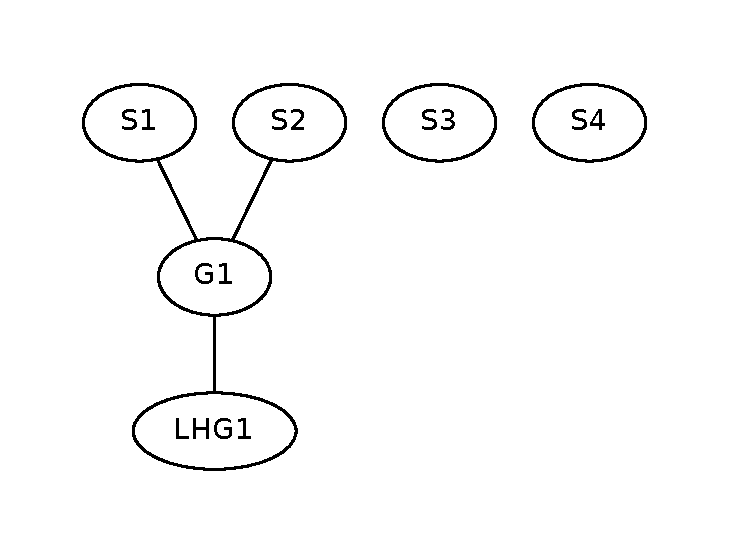
\includegraphics[width=7.0cm]{fig/labgroup/slack_add_1.pdf}        
  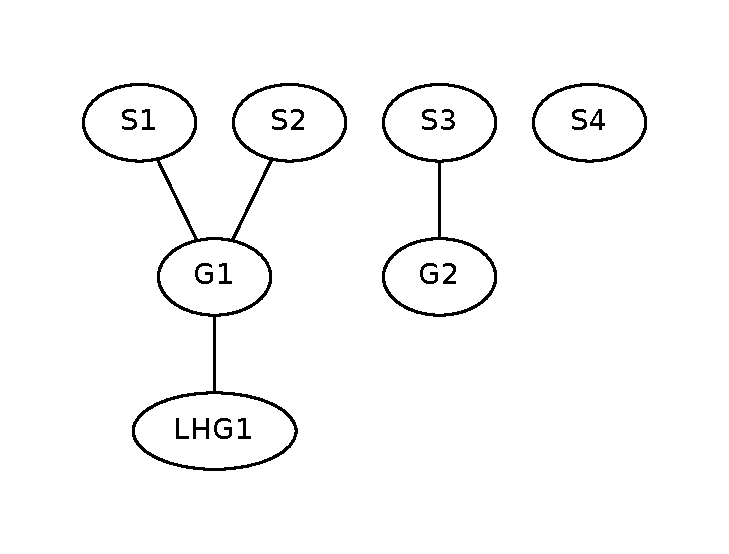
\includegraphics[width=7.0cm]{fig/labgroup/slack_add_2.pdf}        
  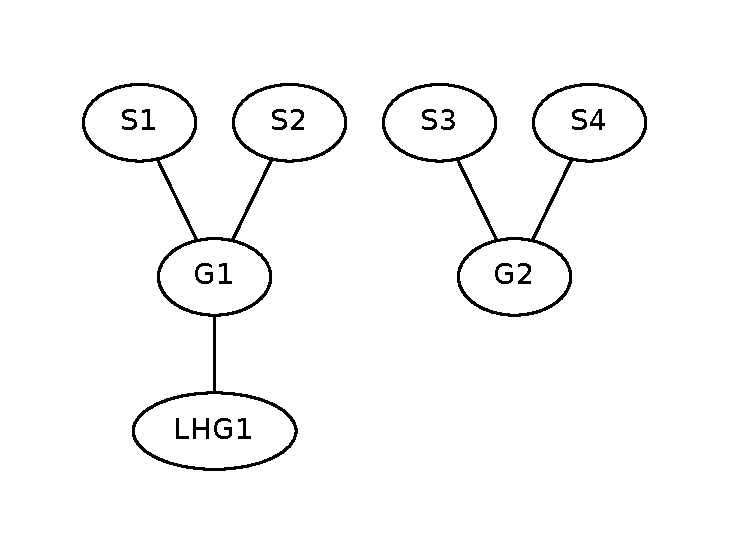
\includegraphics[width=7.0cm]{fig/labgroup/slack_add_2-5.pdf}        
  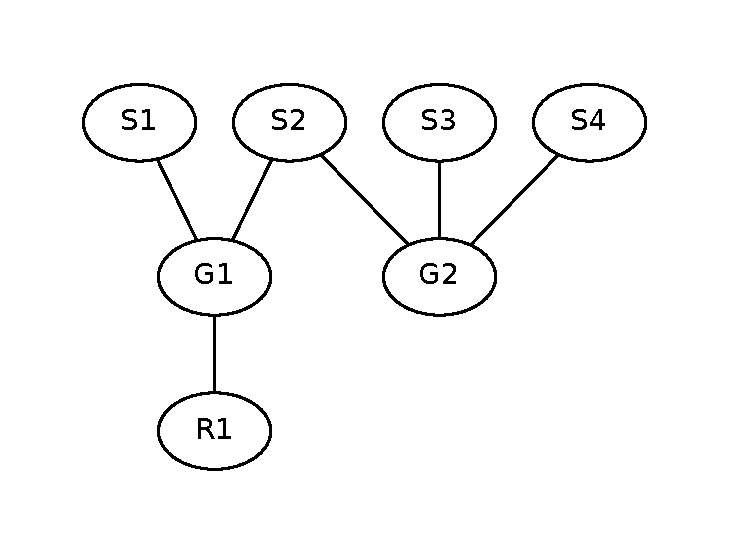
\includegraphics[width=7.0cm]{fig/labgroup/slack_add_3.pdf}        
  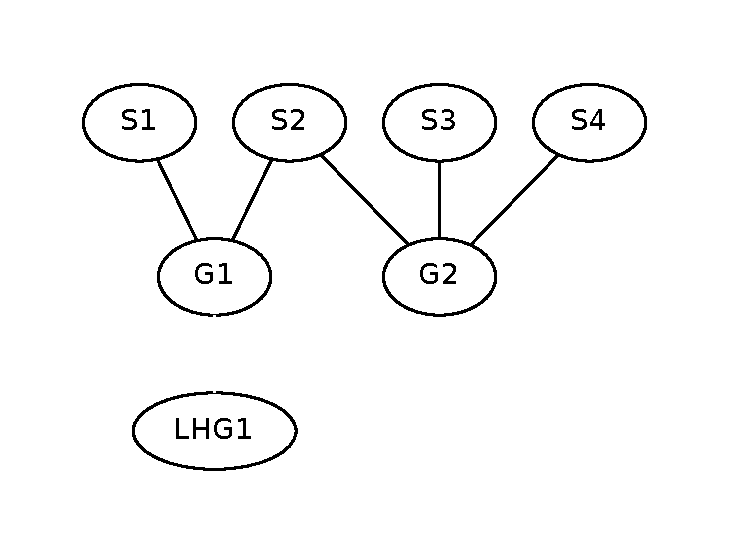
\includegraphics[width=7.0cm]{fig/labgroup/slack_add_4.pdf}        
  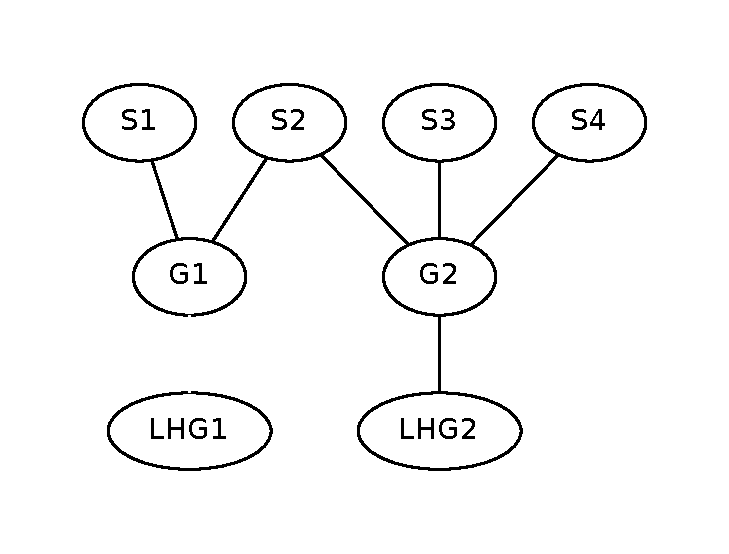
\includegraphics[width=7.0cm]{fig/labgroup/slack_add_5.pdf}        
  \caption[Serie tillstånd rörande labgrupper.]
  {Serie tillstånd rörande labgrupper. Studenterna $S2$, $S3$ och $S4$ vill
  bilda en nya laboraionsgrupp tillsammans (den som blev $G2$) där de ska skapa
  en LHG. Notera hur student $S2$ måste ta bort sin förra LHG innan någon elev
  kan lägga till en LHG i den nya gruppen. Mellan varje figur krävs att någon
  användare gör en åtgärd i waters system.}
  \label{fig:slack_series}
  
\end{figure}

\subsection{Alltid exakt en LHG per laboration ($= 1$)}
Den mindre strikta ($\leq 1$) invarianten ger Water möjligheten att ha ett intuitivt användargränssnitt eftersom ingen student vill se att de gör samma laboration via två olika grupper samtidigt. En striktare variant är dock önskvärd av tekniska skäl. Med en striktare variant behövs till exempel inte hantering av fall då en LHG inte finns, eftersom att den alltid finns. Detta öppnar även upp för att förenkla våra databasförfrågningar, vi kan till exempel få reda på alla laborationer för en student i en kurs genom att “gå” via kopplingarna, eftersom vi har en 1-till-1–relation mellan “laboration-till-grupp”-koppling och laboration per student.

En operationsuppsättning för denna invariant måste även definiera initialtillståndet eftersom det går inte längre att ha studenter utan LHG:s vid kursstart. Operationerna som måste beaktas för denna invariant är fler eftersom tillägg av student eller laboration både är icketriviala. Ifall en student läggs till i en kurs så måste den “direkt” få sina LHG:s. Laborationstillägg måste även se till att varje student får en LHG för den nyligen skapade laborationen. En operation som inte längre kan finnas är att manuellt ta bort en LHG för då skulle invarianten brytas direkt.

\subsubsection{Förslag på implementering}
Invarianten kan  framtvingas genom följande initialtillstånd och operationsuppsättning.

\paragraph{Initialtillstånd}
I början är alla studenter inplacerade i en för varje student unik grupp som kallas “studentens grupp” (förkortat SG i figurerna). Varje student har en sådan grupp som innehåller en LHG till alla laborationer som finns registrerade i kursen. Se figur \ref{fig:strict-initstate}.

\begin{figure}
  \centering
  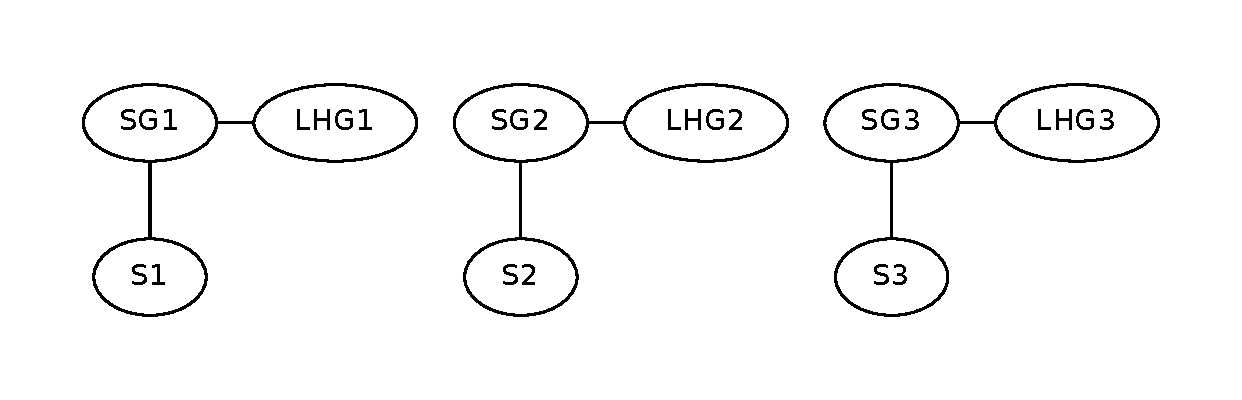
\includegraphics[width=8.0cm]{fig/labgroup/strict_initstate.pdf}
  \caption{Illustration av initialtillståndet i en kurs med 3 studenter}\label{fig:strict-initstate}
\end{figure}

\paragraph{Operationer}
I detta förslag behandlas operationerna “skapa en grupp” och “lägg till en student i gruppen” på samma sätt som i förslaget för den mindre strika invarianten. Att skapa en ny LHG kommer inte ha kräva några förhandsvilkor, studenten behöver alltså inte längre manuellt se till så att LHG:en sätts in genom att ta bort sina egna kopplingar i sina tidigare grupper, istället tar Water bort alla kopplingar som “är i vägen”. Operationen sker mer specifikt på följande sätt:
\begin{enumerate}
  \item För alla medlemmar i gruppen där LHG:en ska läggas till måste deras LHG för den labroationen tas bort.  (De har redan exakt en sådan på grund av invarianten.)
  \item Lägg till LHG:en, nu skall invarianten stämma för gruppmedlemmarna.
  \item Lägg till LHG:en, nu skall invarianten stämma för gruppmedlemmarna.
  \item Borttagningarna i steg ulterkan ha påverkae studenter i andra grupper (FIXA referens se bild). nt påverkade studenterna lägger vi till en LHG i deras egna  tudents laborationsgrupp. De påverkade studenterna kallas för “laborationskamraternas laborationskamrater”. 
\end{enumerate}

Notera att ovanstånde deloperationer sker atomärt, alltså ingenting sker mellan stegen, detta eftersom invarianten blir bruten mellan deloperationerna.

Då en student läggs till en kurs skapas en LHG för varje laboration som placeras i studentens grupp. Då en ny laboration skapas för en kurs så kommer varje student få en LHG för den laborationen insatt i sin egna grupp.

\begin{proof}[Bevis av korrekthet]
I initialtillståndet är invarianten uppenbarligen uppfylld, samt även efter tillägg av student eller laboration. Den enda kvarstående operationen är skapande av en LHG vars beskrivning delats upp i 3 deloperationer. 

Låt mängden A (se figur \ref{fig:strict-proof}) vara samtliga involverade elever som påverkas av operationen, alltså studenten som aktivt lägger till LHG:en, laborationskamraterna till den eleven samt laborationskamraternas laborationskamrater som får sin LHG borttagen i steg 1. 

Låt mängden B vara de elever som är med i laborationsgruppen där LHG:en skapas i steg 2, notera alltså att B$\subseteq$A, notera även att de elever som berörs i steg 3 är A$\setminus$B.

I början antags invarianten vara uppfylld, efter steg 1 så har studenterna i A ingen LHG, efter steg 2 har eleverna i B en ny LHG, endast A$\setminus$B saknar var sin LHG nu, vilket steg 3 åtgärdar. \qedhere
\end{proof}
 
\begin{figure}
  \centering
  \begin{subfigure}[b]{0.5\textwidth}
    \centering
    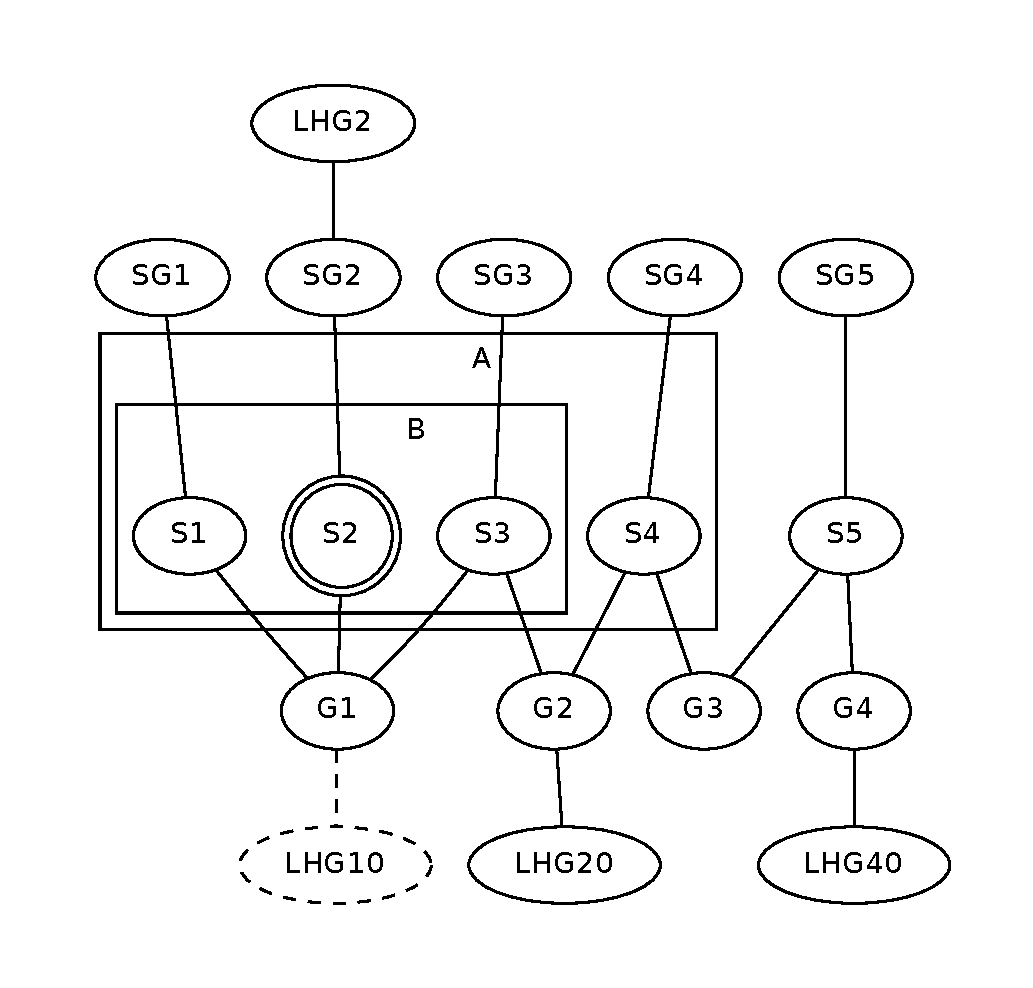
\includegraphics[width=8.0cm]{fig/labgroup/strict_proof.pdf}
    \caption{Situation när $S3$ ska lägga till $R20$}
    \label{fig:strict-proof}
  \end{subfigure}%
        ~ %add desired spacing between images, e. g. ~, \quad, \qquad etc. 
          %(or a blank line to force the subfigure onto a new line)
  \begin{subfigure}[b]{0.5\textwidth}
    \centering
    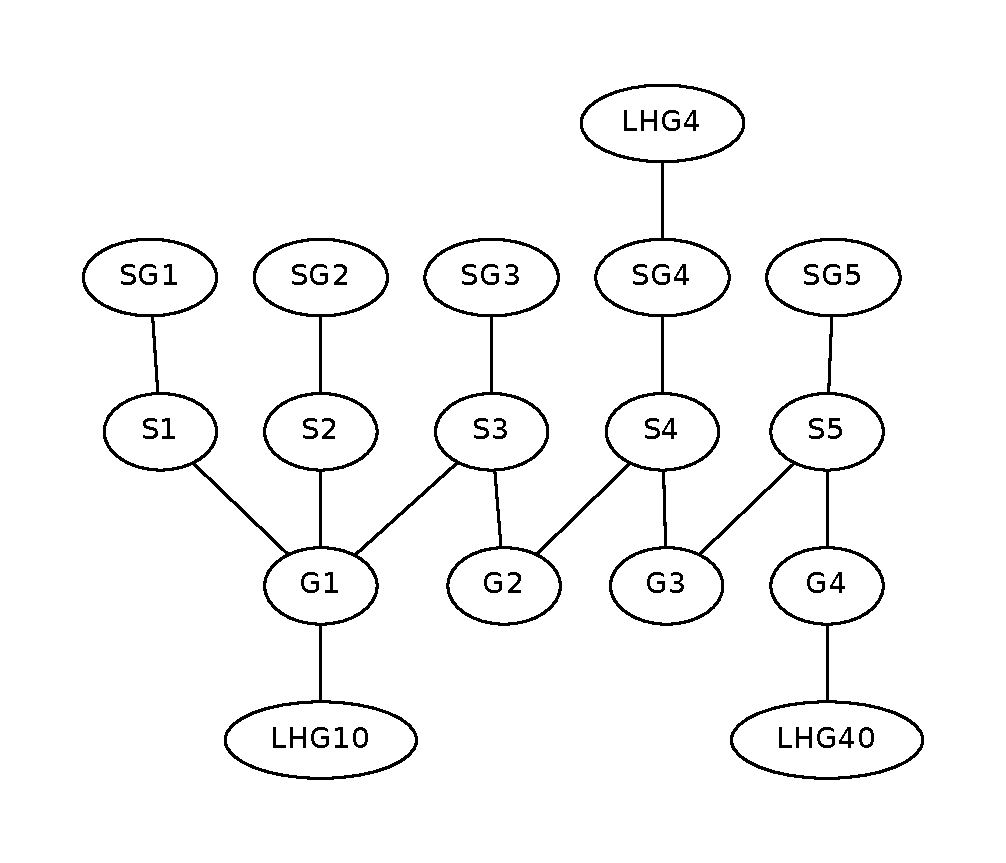
\includegraphics[width=8.0cm]{fig/labgroup/strict_proof_continue.pdf}
    \caption{Situation efter $R20$ lagts till}
    \label{fig:strict-proof-continue}
  \end{subfigure}
  \caption{Före och efter LHG-tillägg (strikt invariant)}\label{fig:animals}
\end{figure}

\subsubsection{Användarperspektiv}
Det ovanstående sättet att skapa en ny LHG innebär att även laborationskamraternas laborationskamrater påverkas av den aktiva studentens operation (se figur \ref{fig:strict-proof-continue}). Detta är givetvis inte bra för de utsatta studenterna. Att samtliga studenter har en egen laborationsgrupp kan vara förvirrande för användare som ser att de redan är medlemmar i en laborationsgrupp som är låst och redan har påbörjat sina laborationer. I gengäld kräver operationen färre steg för en student att påbörja en laboration med en annan laborationsgrupp.

\subsection{Ingen invaraint}
Naturligtvis går det att strunta i att forcera någon invariant. Det blir minimalt med jobb och ingenting behöver bevisas. Nackdelen är att det lätt blir förvirrande för användaren att ha flera aktiva laborationer samtidigt. Vidare krävs fler användaroperationer för att lokalisera sin LHG då användaren inte bara behöver specifiera laboration utan även laborationsgrupp.

\begin{flushright}
  
  \textbf{Beslut}
  
  Vi valde att implementera ($\leq 1$) invarianten. Vi satte hög prestige i ett interface där användare direkt kan klicka på deras laboration utan att först välja laborationsgrupp.
\end{flushright}

\section{Statistik}

Att ha tillgång till statistik från tidigare år hjälper examinatorer att successivt utforma innehållet av laborationer. Till exempel kan en laboration vara för omfattande och då ta för lång tid, vilket resulterar i att de flesta inlämingar kommer in sent, eller inte alls. Det kan också vara av intresse för examinatorn att se hur stor andel av studenterna klarade av en viss laboration.  

Detta kan tas fram genom att implementera attribut i databasen, med vilka statistiken kan tas fram, till exempel ett attribut som innehåller tidpunkten då en grupp gjorde en inlämning.

Datan kan sammaställas i en tabell, med vilken man lätt kan jämföra olika årgångar.

\section{Plagiatkontroll}
På Chalmers upprätthålls den akademiska hederligheten. För inlämningsuppgifter, speciellt programmeringsuppgifter, är det vanligt förekommande att man får samarbeta i någon form. Beroende på inlämningsuppgiftens instruktioner är det ibland godkänt att samarbeta mellan grupper, medan det ibland är av vikt att gruppen lämnar in en unik lösning. (Chalmers tekniska högskola, 2009) I det senare fallet kan det vara tillhanda att automatiskt plagiatkontroll implementeras i inlämningssystemet.

Urkund är ett system för automatisk plagiatkontroll. Texter som behandlas av Urkund jämförs med en bred databas som består av tidigare verk. I dagsläget använder lärare sig utav e-post för att skicka material till Urkund vid misstanke om plagiat. Då Urkund erbjuder ett API till sina kunder (URKUND, 2012), skulle denna process kunna göras betydligt smidigare genom att integrera funktionaliteten direkt i Water.

Ytterligare skulle en intern kontroll av tidigare inlämningar kunna implementeras. För att detta skulle vara möjligt måste samtliga inlämningar som laddas upp till Water behöva sparas i databasen. Därefter skulle en lämplig algoritm för filjämförelse behöva implementeras.

\begin{flushright}
  
  \textbf{Beslut}
  
  Plagiatkontroll nedprioriteras och implementeras inte.
  
\end{flushright}

\chapter{Teknisk problembeskrivning och analys}
I detta kapitel beskrivs viktiga tekniska frågeställningar i anknytning till systemet.
\section{Systemöversikt}
Systemarkitekturen dikteras av systemets syfte. De tekniska utmaningarna består alltså i att impelementera de olika subsystemen. 
Systemet består av flera delsystem: ett versionshanteringssystem, ett webbgränssnitt, logik för inlämningsuppgifter samt en så kallad backend som knyter ihop de olika delarna. Backenden behöver bland annat kunna ta emot inlämningar via versionhanteringssystemet och behandla dem inför rättning och för presentation i webbgränssnittet.
\section{Val av versionshanteringssystem}

Det övergripande valet av versionshanteringssystem stod mellan att använda ett centraliserat system eller ett distribuerat system.

\subsection{Centraliserade system}

Ett centraliserat versionshanteringssystem, hädanefter kallat CVCS (centralized version control system), är ett centraliserat sätt att hantera ändring av data och dokument. Alla ändringar loggas och globaliseras på samma gång med hjälp av en CVCS-klient. Eftersom ändringar centraliseras i samma stund som en logg skrivs så krävs att konflikter i form av merge-problem löses så snart ändringar görs. Detta medför i sin tur att användaren måste ha tillgång till CVCS-servern, vilket oftast kräver internetanslutning.
Enligt O’Sullivan (2009) finns det fördelar med CVCS-system om man hanterar stora binärfiler. Detta eftersom det i CVCS-system ofta finns möjlighet att checka ut en enda commit istället för den kompletta historiken.

Projektgruppen ansåg att det förföll orimligt att tvinga studenterna att ständigt vara uppkopplade mot inlämningssystemet under utvecklingsprocessen. Detta talade emot att systemet skulle byggas på en CVCS-lösning.

\subsection{Distribuerade system}

Ett alternativ till den centraliserade varianten är ett såkallat distribuerat versionshanteringssystem – DVCS (distributed version control system). 
Ett DVCS är ett icke centraliserat system där ändringar kan hållas lokala för att på användarens begäran centraliseras och då även sammanfogas med övriga användares material. Eftersom alla ändringar sker lokalt så ges användaren möjlighet att jobba med experimentell funktionalitet utan att `smutsa ner' den centrala kodbasen. När arbetet sedan är klart kan användaren välja att publicera sitt material. Användaren kan även välja att städa upp sin kodbas genom att  plocka bort eller fixa material innan publicering.
Enligt O’Sullivan (2009) finns det problem med att hantera stora binärfiler i distribuerade system. Stora binärfiler kan till exempel vara texturer i spelutvecklingsprojekt. 

Inom projektgruppen ansåg vi att filer av detta slag torde vara ovanliga inom laborationerna inom data- och it-utbildningar. Därför såg vi  distribuerade system ändå mer lämpliga för våra ändamål.
\begin{flushright}
  
  \textbf{Beslut}
  
  Vi väljer att använde ett distribuerat versionhanteringssystem för att det passar för våra ändamål.
  
\end{flushright}


\section{Plattform}
För de resterande delarna av systemet fanns det flera olika tillvägagångssätt. Det går att exempelvis bygga backend, logik och webbgränssnitt ifrån grunden. Gruppen befarade att detta skulle uppta fler arbetstimmar än vad som fanns till förfogande för projektet.

Ett annat alternativ var att använda sig av en befintligt modul för att visa versionshanterade projekt på webben och bygga resten av webbgränssnittet och backend själva.

En tredje möjlighet som man behövde ta ställning till var att använda befintliga lösningar för så kallad “source code hosting”. Dessa innehåller i regel webbgränssnitt och backend för hantering och presentation av versionshanterade projekt. Systemet skulle byggas ut med logik för inlämningsuppgifter. Tyvärr finns det väldigt få lösningar som bygger på öppen källkod. Ofta är endast delar av systemen öppna. De vanligaste helt öppna exemplen är Gitorious och Launchpad.

Launchpad stöder endast Bazaar medan Gitorious bygger på Git. Därmed finns en koppling mellan valet av source code hosting-lösning och versionshanterare.

Gitorious är byggt i språket Ruby med ramverket Ruby on Rails. Projektgruppen har erfarenhet av ramverket sen tidigare. 

Launchpad är skrivet i Python och Javascript. Systemet kräver i skrivande stund Ubuntu för full funktionalitet (Launchpad, 2009). Systemet är mycket brett och innehåller bland annat moduler för översättning av program, paketering, bugghantering, kollaborativ utformning av kravspecifikationer och system för dynamisk konfiguration av servern.

Oberoende av vilken plattform som skulle användas så fanns det skäl att skala bort den funktionalitet som inte behövs för projektets ändamål. Detta talade emot Launchpad, som innehåller en stor mängd överskottsfunktionalitet.

\section{Licensiering}
Licensiering är i sig ingen teknisk fråga, men för projektet är licensiering starkt sammakopplat med valet av plattform. 

Både Gitorious och Launchpad är licensierade med GNU Affero General Public License (Gitorious, 2012) (Launchpad, 2010) hädanefter kallat GNU Affero GPL. I sin artikel om hur licensen uppkom berättar Vaughan-Nichol (2007) hur licensen ursprunligen kommer ifrån GNU General Public License vilken är en så kallad “Share-alike/Copyleft”-licens.

Konceptet “Copyleft” är resultatet av en  ordlek på den juridiska termen “Copyright”. Copyright nyttjas för att garantera den ursprungliga tillverkaren exklusiva rättigheter för sin produkt. Copyleft, vilket felaktigt kan uppfattas som en motsägelse till Copyright, använder sig utav upphovsrätten för att garantera alla rätten att använda, re-distribuera samt modifiera produkten - så länge som de använder sig av samma licensiering som den ursprungliga produkten. (GNU, 2012)

En produkt som använder sig av GNU Affero GPL måste låta källkoden vara tillgänglig för alla användare av produkten. För webapplikationer som Gitorious och Launchpad innebär detta att källkoden måste vara tillgänglig kostnadsfritt på en server för samtliga användare av applikationen. 
Licenstexten måste göras tillgänglig i samtliga källkodsfiler i systemet. Antingen finns licenstexten i varje fil, eller så finns en central fil som innehåller licenstexten som alla andra filer refererar till (GNU, 2007) 

Sammanfattningsvis innebär detta för kandidatarbetet att oavsett vilken plattform som projektet väljer måste all källkod alltid vara öppen, att vidareutvecklingar av Water alltid måste vara licensierade av GNU Affero General Public License och licensetexten måste alltid gå att finna i eller med hjälp av samtliga filer.

\begin{flushright}
  
  \textbf{Beslut}
  
  Gitorious valdes som grundsystem eftersom kompetens inom Ruby och Ruby on Rails fanns i gruppen och eftersom Launchpad innehåller mycket funktionalitet som inte behövdes i projektet. Eftersom Gitorious är baserad på Git, kommer Git också vara valet av den distribuerade versionshanteringssystemet. Projektet kommer därmed att ligga under GNU Affero GPL-licensen.  
  
\end{flushright}

\section{Tekniska frågor kring validering}

Validering av inlämningar kan ske på olika nivåer – enkel kontroll av formalia, kompilering och testning. 
Att implementera kontroll av formalia, som att vissa filer ska finnas i inlämningen eller att filerna namnges på speciella sätt, är inte svårt. Mer avancerade former av validering ger dock upphov till större tekniska utmaningar.

\subsection{Kompilering}
\label{section:kompilering}

Att en inlämning inte går att kompilera torde i de flesta fall leda till att den blir underkänd. Om systemet kunde testa detta automatiskt skulle det kunna lätta handledarnas arbetsbörda.
För kompilering krävs dock att lämpliga utvecklingsmiljöer finns tillgängliga i systemet. Eventuella externa paket som används måste också läggas till i systemet eller skickas med i inlämningen, om utvecklingsmiljön tillåter det.
Att stöda en stor mängd språk blir arbetsintensivt, speciellt om det uppstår problem kring olika versioner av språk och paket.

Ett realistiskt första steg vore att bara stöda Java. På Chalmers används Java som programmeringsspråk bland annat i kurser som Objekorienterad Programmering, Parallellprogrammering, Datastrukturer och algoritmer och Webbprogrammering (Chalmers tekniska högskola, 2012). Inom branschen i stort har Java länge varit det ett av de största språken – 2012 ligger det på placering två efter C (TIOBE Software, 2012).

Kompilering är tidskrävande och bör därför hanteras asynkront av någon form av kösystem.

\subsection{Unit/Acceptance tester}
Ett ytterligare verktyg för handledare samt examinatorer skulle vara att man i systemet kunde definiera \emph{unit-} och \emph{ acceptancetester}. Detta förutsätter att det går att kompilera kod och lider därför av samma problem som de som beskrivs i avsnitt \ref{section:kompilering}.
\subsubsection{Exekvering av studenters kod}
Att exekvera studenters kod på servern är också förenat med säkerhetsrisker.
För att säkert köra extern kod så skulle systemet behöva upprätta sandboxade miljöer. Helst bör även all beräkningstung validering hanteras asynkront av en köhanterare och ett antal worksers. Ett sådant system är komplicerat och endast färdiga lösningar såsom Jenkins (Jenkins, Meet Jenkins, 2012) eller Bamboo (Atlassian, Bamboo, 2012) är tänkbara.

\subsection{Asynkron validering och deadlines}

Om inlämningar valideras asynkront av systemet kan det uppstå situationer där studenter lämnar in strax innan deadline och får meddelande om retur när tiden har gått ut. Hur dessa situationer ska hanteras måste utredas, förslagsvis i samråd med handledare och lärare.

\section{Water som Git-server}
I allmänhet centraliserar programmerare sitt arbete genom att ha ett
Git-repositorium på en gemensam server (hädanefter kallad \emph{remote}) som
deras organisation tillhandahåller. Programmerarna synkroniserar sitt arbete
via repositorier hos \emph{remote} genom Git-kommandon. Git loggar då in på
\emph{remote} genom SSH-protokollet och skriver programmerarens lokala
ändringar direkt i \emph{remotes} repositorium. Detta var det vanligaste sättet
att centralisera arbete med Git i början av Gits historia (Preston-Werner
2011). Ett nytt sätt att centralisera sitt arbete är att låta någon annan
tillhandahålla remoteservern. Detta är huvudtjänsten som erbjuds av sidor likt
Gitorious och Github och det ska Water också göra.

Sidor som Github har sökvägar till \emph{remote} som egentligen inte matchar
den fysiska platsen för repositoriet i filsystemet. Istället består sökvägarna
utav repo-identifierande komponenter. Till exempel är repositoriumnamnen på
Github unika för varje användare, därför består Githubs repositoriumsökvägar
utav användarnamn samt repositorienamn. När en användare interagerar med ett
repositorium är det hos \emph{remote} sökvägen slås upp till den riktiga
sökvägen, så för användarna kommer ickefysiska sökvägar användas på samma sätt
som fysiska sökvägar.  Water använder samma princip som Github, fast det är nu
en kurs, grupp samt laboration som tillsammans unikt indentifierar
repositoriet. Tabell \ref{tab:repo-paths} visar sökvägar hos
source code hosting-tjänster som använder samma princip.

Eftersom sökvägen identifierar gruppen och inlämningsuppgiften, och eftersom
användaren samtidigt loggas in, går det att avgöra vilka rättigheter användaren
har i sammanhanget. Studenter kan skriva och läsa sin egna kod och handledare
kan endast läsa kod som tillhör grupper kopplade till den kurs handledaren är
handledare i.

\begin{table}
  \begin{tabular}{ | p{5cm} | p{8cm} |}
    \hline
      fysisk sökväg med SSH & \url{ssh://user@domain/real/folders/repo-name.git} \\ \hline
      repoidentifierande sökväg (SSH på Github) & \url{git@github.com:user/project-name.git} \\ \hline
      SSH på Gitorious & \url{git@gitorious.org:my-organization/my-repo.git} \\ \hline
      https på Github & \url{https://user@github.com/user/project-name.git} \\ \hline
      https på Gitorious & \url{https://git.gitorious.org/my-organization/my-repo.git} \\ \hline
      tänkbar repoidentifierande sökväg för Water & \url{https://repos.water.com/courses/4/lab_groups/1/labs/2.git} \\
    \hline
  \end{tabular} 
  \caption{Exempel på repositoriumsökvägar hos source code hosting-sidor}
  \label{tab:repo-paths}
\end{table}


\subsection{HTTP-protokollet}
Nämnt är att SSH var det vanligaste protokollet för att kollaborera på samma
repositorium, oavsett om man har en egen server eller använder tjänster likt
Github. Git har även ett eget protokoll, men det är inte intressant för oss
eftersom det är bara för läsning och det inte är möjligt att modifiera
fjärrepositorium via det (Chacon, 2009). Ett attraktivt alternativ till SSH är
HTTP, det är enklare för användare att komma igång via HTTP.  Med SSH så måste
användarna sätta upp SSH-nycklar, det försvårar användandet av Water via en
kommandoradsklient.  Vidare har många brandväggar portarna som HTTP och HTTPS
(säker HTTP) öppna (Chacon, 2010), vilket minskar risken för brandsväggsproblem
när Water kontaktas via en konsolklient.

I Gitorious finns redan stöd för SSH. Implementationen måste ändras för att
stödja Waters repositorieidentifierade sökvägar. För smart HTTP finns en mer
uppdaterad färdig server, Grack.  Eftersom Grack är Rackbaserat är det enkelt
att göra egna tillägg till servern (Rubyforge, 2012). Komponenter som skriver
om repoidentifierande sökvägar till fysiska sökvägar samt autentiserar och
bestämmer rättigheter för användaren går alltså att lägga till för Water.

\begin{flushright}
  
  \textbf{Beslut}
  
  Vi utesluter SSH och använder HTTP med Grack eftersom att det är modernare och minskar kodmängden vi behöver underhålla.
  
\end{flushright}

\section{Uppladdningsprocessen via webbgränssnittet}

Ett led i arbetet med att göra Water mer användarvänligt än Fire är att förbättra uppladdningsprocessen. I Water bör det därför vara möjligt att ladda upp flera filer på samma gång, utan att behöva paketera dem i en arkivfil. Uppladdnings ska även vara möjlig till olika positioner i ett filträd, istället för bara i roten.

\subsection{Uppladdning på olika positioner i filträdet}

För att möjliggöra uppladdning på lika positioner i filträdet måste det vara möjligt att navigera i det. Någon entitet måste dessutom hålla reda på den nuvarande sökvägen.

\subsection{Uppladdningsprocessens två skeden}
Uppladdningsprocessen består av två faser. Först laddas filerna upp till servern. Därefter läggs de till i ett lämpligt repositorium. Dessa steg går i princip att utföra i ett enda anrop. Detta gör det dock mycket komplicerat att ladda upp filer till olika sökvägar i filsystemet, eftersom gränssnittet  måste ge användaren möjlighet att förbereda många uppladdningar på olika noder i filsystemet innan samtliga uppladdningar skickas på samma gång tillsammans med samtliga sökvägar.

Ett alternativ är att filuppladdningen skiljs från repositorieoperationerna. Klienten laddar upp filer till servern som returnerar någon form av pekare till filerna i ett temporärt förvar. Klienten kan ladda upp grupper av filer som hör till en viss sökväg, navigera till nästa position i filträdet och ladda upp filer där. Till sist läggs samtliga filer till i repositoriet med ett separat anrop som innehåller pekare och sökvägar. Den sista operationen har projektgruppen valt att kalla en \emph{CommitRequest}.

\subsection{Kvittering av uppladdade filer}

Det som komplicerar ett system med separat filuppladdning och \emph{CommitRequest} är att klienten måste hålla reda på de filer som har laddats upp. Den naiva lösningen är att lagra filnamnen i klienten och returnera dem från servern för kvittering av uppladdningen. Problem uppstår dock om klientens webbläsare och webbservern använder inkompatibla teckenkodningar. Kvittensen matchar i det fallet inte det filnamn som lagras i klienten. 
Detta kan lösas med hjälp av att klienten kör filnamnen genom en \emph{hashfunktion}, och sparar undan dess \emph{hashar}. När servern sedan rapporterar vilka filer som har blivit uppladdade är det \emph{hasharna} som jämförs.

\subsection{Filnamnskrockar i temporär lagring}
Risken med den temporärlagring som används i en delad uppladdningsprocess är att filnamnen på uppladdade filer krockar och att filer därför skrivs över. För att undvika detta kan även servern använda en \emph{hashfunktion} för att ge de temporära filerna ett nytt namn.

\subsection{CommitRequest-API}
Ett API bör specificeras för Git-manipulationer via webbgränssnittet. Förutom tillägg av filer ska APIt även stöda skapande av mappar och borttagning av filer och mappar.

\begin{flushright}
  
  \textbf{Beslut}
  
  En tvådelad uppladdningsprocess används.
  
\end{flushright}

\section{Rollhantering}

\subsection{Roller i databasen}

En webbapplikation behöver i allmänhet hantera användare. Dessa användare organiseras ofta i en hierarki som specificerar vad varje användare kan och inte kan göra. Detta kan lösas på ett flertal sätt antingen i \emph{databas-lagret} eller i \emph{modell-lagret}.

I \emph{databas-lagret} kan det lösas genom att lägga till en kolumn i användartabellen där bitvis eller 
operatorn används för att kombinera flera roller, detta är dock inte kongruent med en \emph{normaliserad databas} som beskrivs i kapitel \ref{sec:databasen}. En annan databas-lösning är att ha en separat tabell med alla tillgängliga roller och en tabell som kopplar ett godtyckligt antal roller på ett godtyckligt antal användare, dvs en n-m relation, detta är kongruent med en \emph{normaliserad databas} men databasoperationerna för att hämta en användares roller blir mer komplexa.

Genom att lägga rollhanteringen i \emph{modell-lagret} blir applikationen mer \emph{databas-agnostisk} då den inte kräver avancerade funktioner av databasen. En sådan lösning kan implementeras med en användartabell som håller information alla användare behöver och en separat tabell för varje roll som har en koppling till användartabellen. Att lägga all logik i \emph{modell-lagret} underlättar för framtida utvecklare då de inte behöver gå igenom hela \emph{databas-schemat} för att förstå rollhanteringen. Nackdelen med detta är att rollerna inte blir dynamiska, för att lägga till en roll krävs det att en ny tabell läggs till i databasen.

\subsection{Roller i Routes}

För att behålla \emph{REST}-egenskaperna vid en implementation av roller behövs det ett sätt att avgöra vilken roll som är aktiv utan att skapa en cookie. Detta kan lösas genom att placera alla sökvägar inom en namnrymd – ett \emph{scope} - som indikerar den aktiva rollen. Användaren kan ha flera roller, även inom samma kurs, men webbapplikationen vet alltid vilken den aktuella rollen är eftersom den går att utlösa ur sökvägen. På detta sätt är applikationen fortfarande tillståndslös till den mån att man behöver logga in.
Exempel på en \emph{scopad} \emph{route} som visar en students kurser är |/student/courses| där courses är \emph{scopad} under student.

Det finns dock sökvägar som inte bör ligga inom namnrymden för en roll. Exempel på detta är inloggningssidor och allmänna inställningaspaneler. Detta leder till specialfall i routingsystemet. Komplexiteten hos routingen kan öka avsevärt.

\begin{flushright}
  
  \textbf{Beslut}
  
  Roller implementeras som separata svaga entiteter. Rollhanteringen i webbapplikationen sköts med \emph{scopes} i sökvägarna.
  
\end{flushright}

\section{Strukturering av Javascript och CSS}

Water kommer att innehålla stora mängder Javascript och CSS. För att systemet ska vara lätt att vidareutveckla och underhålla behöver strategier tas fram för strukturering av dessa filer.

\subsection{Prestanda kontra läsbarhet och utvecklingsbarhet}

Under utvecklingsfasen, och med tanke på att systemet bör vara lätt att underhålla och vidareutveckla, är det önskvärt att klientkoden struktureras på samma sätt som traditionell kod. Detta innebär i regel att koden delas upp i separata filer och mappar enligt funktion eller några andra lämpliga kriterier.

Språk som CSS och javascript har dock i regel inga include-direktiv eller liknande mekanismer för att inkludera eller referera till kod från andra filer. Samtliga källkodsfiler måste istället länkas in en åt gången i HTML-dokumentet. 
Webbläsaren hämtar sedan filerna genom att göra ett separat anrop per fil till servern. Anropen går till viss del att göra parallellt, men HTTP 1.1-specifikationen (IETF, 1999) rekommenderar att webbläsare begränsar antalet parallella överföringar till två. Detta beror på att ett stort antal (nästan) samtidiga anrop riskerar att överbelasta webbservern. Resultatet blir att filerna överförs i serie. Av Breit (1998) framgår det att detta är dåligt ur prestandasynpunkt eftersom varje nytt anrop ger upphov till olika handskakningsförfaranden som tar i anspråk bandbredd och processorcykler. 

Det är alltså mer effektivt att överföra en given datamängd som ett enda stort paket än som en större mängd små paket. Det är därför önskvärt att konkatinera ihop CSS- och javascriptfiler till ett litet antal större källkodsfiler. Detta står dock i direkt konflikt med kravet på strukturering och uppdelning av koden.

För att ytterligare snabba upp hämtning av resurser går det att använda olika tekniker för att minska storleken på javascript och CSS. Detta åstadkommes bland annat genom att eliminera alla onödiga whitespaces och genom att göra variabel- och funktionsnamn så korta som möjligt. Processen kallas för minifiering. Den minskar laddningstiderna men gör koden oläsbar av människor. Minifiering sker dock i samband med produktssättning – under utvecklingstiden behandlas icke-minifierad kod.

\subsection{Konkatineringsverktyg - en möjlig lösning}
Ett sätt att dra nytta av både välstrukturerad källkod och olika prestandaförbättringar är att använda ett verktyg som låter programmeraren dela upp källkodsfilerna under utvecklingsfasen, men som konkatinerar dem på lämpligt sätt då applikationen sätts i produktion. 
Verktygen är oftast plattformsberoende. Eftersom Water kommer att bygga på Ruby on Rails kommer alternativen för den miljön att utforskas. 
De mest populära verktygen för Ruby är Sprockets och Jammit. Båda erbjuder konkatinering och komprimering av Javascript och CSS. Båda erbjuder även hjälpmedel för cachning av resurser. Små skillnader finns i syntaxen som används för att styra hur filerna konkatineras.
Sprockets är välintegrerat i Ruby on Rails genom ramverkets system för assethantering - asset pipeline.

\begin{flushright}
  
  \textbf{Beslut}
  
  Sprockets väljs som konkatineringsverktyg på grund av den goda integrationen i Ruby on Rails.
  
\end{flushright}

\subsection{Strukturering av avancerade Javascriptapplikationer - \emph{MVC}-modell i klienten}
I takt med att Javascriptapplikationer i webbklienten blir mera avancerade uppstår problem med struktur och underhållbarhet. En anledning kan vara historisk - Javascript har traditionellt använts i form av små ostrukturerade kodsnuttar på olika ställen i en webbsida. Möjlighet att använda ett tämligen objektorienterat arbetssätt finns i Javascript tack vare prototypsystemet (ECMA-262, sektion 4.2.1, 2011), men detta används sällan. Istället skrivs kod i monolitiska filer i ett i närmast imperativt idiom.

En möjlig lösning är att använda sig av \emph{MVC}-modellen även i Javascriptkoden i webbklienten. Domänlogik och datahantering enkapsuleras i modeller. Vyer observerar förändringar i modeller och renderar data. I klassisk \emph{MVC} tar en controller emot anrop från modell och vy och sköter kommunikationen mellan dem. Event-systemet i Javascript gör emellertid att vyer i många fall kan kopplas direkt till modellobjekt, vilket gör att controllerns roll blir snävare i klient-\emph{MVC}. I klienten används controllern oftast bara för att knyta sökvägar i sökvägens \emph{hash fragment} till händelser som hanteras av modellerna. Därför brukar den ibland kallas för router i sammanhanget.

\emph{MVC}-stöd i klienten löses enklast genom färdiga bibliotek för ändamålet. Två av de vanligaste alternativen är Spine.js och Backbone.js.
Båda erbjuder mogen \emph{MVC}-funktionalitet. De erbjuder prototyper, en form av superklasser, som programmeraren kan använda för att skapa sina vyer, modeller och controllers. Skillnaderna hör till de övriga egenskaperna. 
Backbone.js är bättre integrerat med jQuery. Exempel på detta är hjälpmetoder i vyer för att hämta vyns HTML-element som ett jQuery-objekt. Backbone.js är skrivet i vanlig Javascript, medan Spine.js är skrivet i och anpassat för CoffeeScript, ett språk som kompileras till Javascript. Backbone kan dock användas med CoffeeScript och Spine kan användas med vanlig Javascript. Backbone erbjuder Collections, som är en samling modeller. Den huvudsakliga fördelen med Collections är att Backbone kan popularisera en Collection och uppdatera enskilda modeller i den med hjälp av en enda sökväg, förutsatt att serverns sökvägar följer \emph{REST}-standard.

Sammanfattningsvis går det att säga att valet av bibliotek beror på tycke och smak.

\begin{flushright}
  
  \textbf{Beslut}
  
  Backbone.js används som \emph{MVC}-bibliotek i klienten, på grund av jQuery-integrationen och på grund av att det finns tidigare erfarenhet av biblioteket inom gruppen.
  
\end{flushright}

\section{Databasen}\label{sec:databasen}

Valet av databas står mellan MySQL och PostgreSQL, de största aktörerna på marknaden inom fria relationsdatabaser (Mlodgenski 2010).

I en webbapplikation där databastranskationerna sker slumpmässigt 
med korta intervall är det en fördel att ha en \emph{normaliserad} databas (Wang 2010). 
Att en databas är \emph{normaliserad} innebär att den har minimalt med redundans och bättre dataintegritet.

En databas kan normaliseras till flera nivåer, i en typisk webapplikation är det vanligt att
normalisera till den tredje eller fjärde nivån. 
Normalisering innebär att den måste följa vissa specifikationer, 
när databasen följer dessa specifikationer sparas ingen data mer än en gång 
och restriktionerna minskar risken för att  felaktig data sparas.

En \emph{normaliserad databas} kan inte garantera att ingen felakig data sparas, modell-lagret måste fortfarande implementeras korrekt. Att implementera ett \emph{modell-lager} för en \emph{normaliserad databas} kan leda till mer avancerade SQL-operationer, en implementation för en icke-normaliserad databas kommer ha mindre komplexa operationer men den kommer behöva göra fler operationer för att uppdatera alla referenser.

\subsection{Datavalidering}
För att behålla dataintegriteten i databasen behöver data valideras innan det sparas, denna validering kan ske antingen i \emph{databas-} eller \emph{modell-lagret}.
Det är inte bättre att implementera det på det en stället än de andra men vanligast är ändå att lägga de enklaste valideringarna i databasen och resten i modell-lagret. För att implementera valideringar i databasen används \emph{constraints}, \emph{triggers} och till viss mån \emph{foreign keys}. Här kommer valet av \emph{DBMS} in i bilden då alla inte har fullt stöd för \emph{constraints}.
Det är svårare att underhålla logik i \emph{databas-lagret} då en ändring på en tabell kan påverka flera \emph{triggers}, detta kan leda till en problematisk felsökning.
När målet är en fullständigt \emph{databas-agnostisk} applikation måste då alla valideringar ligga i modell-lagret. 

\subsection{Rekursiv borttagning av poster i databasen}

I modellen är det naturligt att vissa entiter är beroende av andra, det vill säga att de är svaga entiter. Till exempel så bör en laboration inte existera om den inte tillhör någon kurs och därför bör också laborationen tas bort om kursen den tillhör tas bort. 

Det finns olika sätt lösa problemet. Många \emph{DBMS} har cascade-delete funktionalitet som kan läggas till i entiteterna på \emph{databas-lagret}, vilket skulle få den önskade effekten. Det finns också en Rails-specifik metod som heter dependent-destroy, som har samma effekt som cascade-delete, men som verkar i modell-lagret.

Med cascade-delete används kan det uppstår problem om systemet byter databas, i och med att olika \emph{DBMS} skiljer sig i funktionalitet.

En annan orsak till att använda dependent-destroy är att det blir lättare för en Rails-utvecklare att ta över projektet, eftersom att använda metoden är en konvention inom Railskretsar.

Kandidatgruppen anser också att det viktigt att vara konsekvent med på vilken nivå valideringar, och funktionalitet som rekursiv borttagning läggs, för att göra systemet lättare att underhålla, och vidareutveckla.   

\begin{flushright}
  
  \textbf{Beslut}
  
  Vi valde att implementera rekursiva borttagningar i \emph{modell-lagret} med hjälp av dependent-destroy.
\end{flushright}

\section{Specialiserad kommunikation mellan webbserver och klient}

En webbapplikation med en avancerad klientdel kan drabbas av problem som beror på begränsningar i de traditionella internetteknologierna.

\subsection{Traditionell kommunikation på webben}

För kommunikation mellan en webbserver och webbklient används traditionellt synkrona envägsanrop via HTTP-protokollet. HTTP-protokollet hindrar i sig inte tvåvägskommunikation, men relationen servern och klienten är fast - det är klienten som inleder kommunikationen med anrop och servern svarar. Servern kan inte på eget bevåg kontakta klienten (IETF RFC 2616, sektion 1.4, 1999). Tvåvägskommunikation är alltså inte möjligt, trots att det är ett vanligt behov i avancerade webbapplikationer.

\subsection{Problem med långa bearbetningstider}

Nära relaterat till frågan om tvåvägskommunikation är problemet med långa bearbetningstider.

Långa bearbetningstider kan att uppstå i projektet, till exempel när uppladdade filer ska läggas till i ett Git-repositorium. 

Om ett anrop till servern tar länge att behandla uppstår två viktiga problem:
Antalet öppna uppkopplingar är begränsat. Anrop med långa bearbetningstider sänker därför snabbt serverns förmåga att ta hand om alla inkommande anrop. Det är därför viktigt att webbservern kan avsluta arbetet med ett givet anrop så fort som möjligt. 
Vid vanliga synkrona anrop låses webbläsaren och därmed användargränssnittet tills servern svarar. Även om anropet i fråga egentligen skulle kunna påverka endast en avgränsad del av webbappliktionen så  förlorar användaren hela sin möjlighet att interagera med den i väntan på svaret. Dröjer svaret tillräckligt länge kommer webbläsaren att ge upp och tolka händelsen som att webbservern har slutat fungera.

För att avlasta webbservern bör alltså tyngre bearbetning flyttas till externa processer. Dessa externa processer behandlas i större detalj i avsnittet om köhanterare.
Anropet kan i detta fall behandlas snabbt eftersom webbservers enda uppgift är att vidarebefordra arbetet. Problem uppstår dock i webbklienten om systemet använder synkrona anrop och avlastar bearbetningen till externa processer, eftersom webbservern besvarar anropet direkt efter att delegeringen har skett – alltså innan det önskade arbetet har slutförts.
Om klienten däremot kunde göra ett första anrop till servern för att inleda bearbetning, och sedan kunde ta emot anrop från servern när bearbetningen är klar, så skulle både klientens och serverns behov tillgodoses. Kommunikationen blir asynkron. Denna form av kommunikation är dock inte möjlig på grund av webbserverns rigida relation till klienten.


\subsection{Möjliga lösningar}

\subsubsection{Polling} är en den mest naiva lösningen och går ut på att klienten gör anrop med jämna mellanrum till servern för att ta reda på om arbetet är utfört. Polling är lätt att implementera med grundläggande teknologier som HTTP, HTML och Javascript. Nackdelen är att servern riskerar att överbelastas av en stor mängd onödiga anrop. För att minska belastningen kan intervallet mellan varje anrop förlängas. Detta leder dock till att användaren upplever att systemet är långsammare, eftersom arbetet kan ha slutförst alldeles i början på ett vänteintervall.

\subsubsection{Long polling} är en vidareutveckling av polling. Servern tar emot klientens anrop och kontrollerar om arbetet är klart. Om inte så lagrar servern anropet under ett kortare tidsintervall. Om arbetet slutförs under detta intervall så svarar servern direkt till klienten. Om arbetet inte slutförs under intervallet svarar servern med en instruktion till klienten att skicka ett nytt anrop. Detta enligt beskrivning av Mesbah och van Deursen (2008). 

Jämfört med polling undviker klienten risken att behöva vänta ett helt uppdateringsintervall innan den får meddelande om slutfört arbete. Servern behöver i sin tur ta emot färre anrop. Servern blockeras dock under long polling-intervallet.

Polling och long polling är bygger alltså på befintlig HTTP-teknologi och utgör egentligen inte en ren tvåvägskommunikation. För att uppnå detta krävs nya teknologier.

\subsubsection{Websockets}
IETF RFC 6544 (2011) beskriver WebSocket-protokollet:
The goal of this technology is to provide a mechanism for browser-based applications that need two-way communication with servers that does not rely on opening multiple HTTP connections (e.g., using XMLHttpRequest or <iframe>s and long polling)
WebSocket-protokollet möjliggör tvåvägskommunikation mellan server och klient genom en enda TCP-uppkoppling. Handskakning sker dock via modifierade HTTP-anrop för att bibehålla en viss bakåtkompatibilitet.
WebSocket-protokollet är emellertid ännu bara ett förslag. Någon färdig standard finns inte och webbläsarstöd finns i regel bara i tämligen nya versioner.

\subsection{Den optimala lösningen: WebSockets med fallback}
På grund av att ingen standard är fastställd och det varierande webbläsarstödet är det viktigt ur användarvänlighetssynpunkt att även stöda de äldre teknikerna för tvåvägskommunikation.
Socket.IO och Faye är två möjliga lösningar. Båda består av en serverdel och en klientdel. Båda erbjuder en serverdel skriven i Javascript för node.js. Faye erbjuder dock även en server skriven i Ruby.
Båda använder WebSockets, Adobe Flash Sockets och olika metoder av polling och long polling för att erbjuda stöd för gamla webbläsare samtidigt som moderna webbläsare kan utnyttja de senaste teknikerna.

\subsection{Säkerhet}
Ett problem som uppstår, oavsett valet av mjukvara, är sändningsrättigheter mellan server och klient. Idén med socket-protokollet, som tidigare nämns är att möjliggöra tvåvägskommunikation mellan klient och server. Servern och klienten kan i princip när som helst sända vilka paket som helst till vilken nod som helst. Det enda klienten och servern behöver veta om är vilken kanal som informationen ska skickas på och vilken socket-server som ska agera nav. Risken finns att en obehörig person väljer att skicka ett meddelande till alla uppkopplade klienter i nätverket.

Varken System.IO eller Faye innehåller någon inbyggd säkerhetsfunktionalitet. Vi måste hitta ett bibliotek eller implementera säkerhetsfunktionerna själva.

\begin{flushright}
  
  \textbf{Beslut}
  
  Faye används för att leverera tvåvägskommunikation mellan server och webbläsare. Faye väljs eftersom det erbjuder en server skriven i Ruby, som är projektets huvudspråk. Kommunikationen säkras med hjälp av biblioteket SecureFaye.
  
\end{flushright}


\chapter{Metod}

\section{Intervjuer}

Intervjuer utfördes med olika personer med anknytning till Fire. Intervjuerna var icke-strukturerade till sin natur. 

\section{Iterativ utveckling}

Projektet delas upp i två eller fler iterationer. Under den första iterationen
utvecklas en fungerande prototyp med de funktioner som utgör absoluta krav.
Under den andra och tredje iterationen utvecklas övriga funktioner. Mellan
iterationerna utvärderas produkten.

Iterationerna delas i sin tur upp i mindre subiterationer på två veckor där
fokus ligger på enskilda  funktionella områden. Projektet har brutits ned i
följande funktionella områden: Registrering, Inlämning, Administration,
Kommunikation och Rättning. En subiterationscykel börjar med definitioner av
deluppgifter och slutar med redovisning och utvärdering.

\section{Prioriteringar}

Projektet delas upp i tre prioritetsnivåer, där funktioner på den första nivån är absoluta krav som ska realiseras under den första iterationscykeln.

\subsection{Första prioritet}

\begin{itemize}
\item Som en student ska man kunna registrera sig på Water
\item Som en student ska man kunna lämna in sin laboration via versionshanterare och webbgränssnitt
\item Som en student ska man kunna få sin laboration rättad
\item Som en handledare ska man kunna rätta laborationer
\item Som en examinator ska man kunna skapa en kurs
\item Som en examinator ska man kunna skapa en laboration
\item Som en examinator ska man kunna modifiera sina befintliga kurser och laborationer
\item Som en examinator ska man kunna skriva ut LADOK-vänliga listor
\item Som en examinator ska man kunna delegera vissa administrativa rättigheter till handledare
\end{itemize}

\subsection{Andra prioritet}

\begin{itemize}
\item Som en student ska man kunna ha en interaktiv dialog med sin handledare med hjälp av systemet
\item Som en handledare ska man med hjälp av systemet kunna få stöd till rättning i form av enkla valideringar
\item Som en examinator ska man få tillgång till aktuell statistik
\end{itemize}

\subsection{Tredje prioritet}

\begin{itemize}
\item Undersöka möjligheten att skriva betyg direkt till LADOK
\item Undersöka möjligheten till automatisk plagiatkontroll
\item Undersöka möjligheten att validera inlämningar med hjälp av unit/acceptance tests
\item Undersöka anonym rättning
\end{itemize}

\section{Projektorganisation}

Gruppen använde en platt organisation. Inga fasta positioner delades ut.
Arbetsuppgifter registrerades som \emph{issues} på \emph{source code hosting}-tjänsten Github,
där koden också förvaras. Dubbelarbete kunde undvikas genom att personen som
arbetade med ett visst problem designerade sig själv som \emph{assignee} på den
relevanta issuen. Commits kan knytas till issues vilket gör det möjligt att
spåra det arbete som utförs på området. Issues utan assignees eller commits
antyder att arbetet har stagnerat.

\section{Testning}
En viktig del i utvecklingen av Water har varit verifieringsprocessen i form av tester. Då gruppen består av personer från olika bakgrunder med olika förkunskaper så är det viktigt att koden som skrivs kan verifieras av både skribenten och övriga utvecklare inom gruppen.

\subsection{Testmetoder}
Tester kan skrivas på lite olika sätt och enligt lite olika konventioner. Några utav dem är TDD (Test Driven Development), RDD (Readme Driven Development), BDD (Behavior Driven Development) och TAF (Test After Programming).

Ett utav de vanligare sättet att skriva tester på, enligt tidigare erfarenhet från gruppen, är TAF. Principen är att testerna skrivs efter de att koden har implementerats.

\subsection{Testramverk}
Språket Ruby har ett flertal testramverk som är under aktiv utveckling, tre utav de större är MiniTest, RSpec och TestUnit. Valet av ramverk är viktigt, främst då ramverket är svårt, om inte nära inpå omöjligt att byta efter att utvecklingen har påbörjats.

Några utav de faktorer som spelade in vid valet är
\begin{itemize}
    \item Dokumentation – hur enkelt är det att läsa sig in på ramverket
    \item DSL – hur lättläst är test-koden som skrivs av utvecklaren
    \item Förkunskaper inom gruppen
    \item Rails-stöd
    \item Exekveringstid
\end{itemize}

Rubys TestUnit, som till sitt DSL är mest likt Javas JUnit, är flera gånger snabbare än RSpec, men är inte praktiskt att använda då DSL:et är förhållandevis oläsbart. Rubys möjlighet till metaprogrammering gör det möjligt att designa lättlästa DSL:er. Vi kan därför förvänta oss ett bättre designat API, vilket gör att TestUnit fallet bort.

MiniTest, som förövrigt är standardtestramverket i Rails sedan 2008 (Rails Webblog, “MiniTest”, 2008), är likvärdigt med RSpec både när det gäller läsbarhet, DSL-uppbyggnad och körningstid. Det fattas kompetens inom gruppen för biblioteket, vilket tillslut gjorde att valet tillslut föll på RSpec.

RSpec har fullt stöd för Rails, har ett lättläst DSL (se exemplet nedan) och är mycket bra dokumenterat. Ett flertal personer inom gruppen har även kunskap om testramveket.

Nedan följer ett exempel på hur RSpec skulle kunna tänkas användas för att testa en bil-klass.

\begin{lstlisting}[language=Ruby]
it "should_have_3_wheels" do
  car.should have(3).wheels
end

it "should_not_be_roadworthy" do
  car.should_not be_roadworthy
end
\end{lstlisting}


\begin{flushright}
  
  \textbf{Beslut}

  Vi väljer att använda RSpec eftersom den är lättläst, bra dokumenterat och för att det finns kunskap om testramverket inom gruppen sen tidigare.
\end{flushright}

\subsection{Vad testas?}
Det vore optimalt med 100\% test-täckning, i praktiken har inte detta varit möjligt.

Vi påbörjade utvecklingen av Water genom att strukturera upp och implementera en databas, var vid modellagret i MVC-modellen applicerades. Under utveckingen av modellerna så användes BDD-metoden för att bygga och strukturera upp testerna. 

Ett problem vid modelltesting är popularisering av objekten som ska testas. En lösning är att skapa s.k fixtures. Fixtures är färdigpopulariserade och validerade objekt som används vid testing.

User-modellen innehåller ett namn, lösenord och en epost-adress. Problem uppstår när utvecklaren ska testa specifika attribut, till exempel existensen av namn. De vi vill göra är att modifiera specifika attribut, men behålla resterande fält för att se vilken effekt våra ändringar har.

Rubygemen FactoryGirl enkapsulerar factory-konceptet och gör det möjligt att göra just detta. Exemplet nedan illustrerar en user-modell som är färdigpopulariserad och redo att använda.

\begin{lstlisting}[language=Ruby]
FactoryGirl.define do
  factory :user do
    name "Pelle"
    email "pelle@student.chalmers.se"
    password "secret"
  end
end
\end{lstlisting}

När factoryn sedan ska användas i testerna så kan vi enkelt välja att plocka bort och ändra attribut utan att behöva modifiera eller ens lägga till övriga attribut. I exemplet nedan är det inte tillåtet för en user att heta Gustav, men andra namn är tillåtna. Om implementationen är rätt så kommer båda testerna passera.

\begin{lstlisting}[language=Ruby]
build(:user, name: "Gustav").should_not be_valid
build(:user, name: "Lasse").should be_valid
\end{lstlisting}

Efter modellen föjer implementeringen av vyn och kontrollern (VC i MVC). VC är svårare att testa, jämfört med M, då VC innehåller två lager. Vyn är som bekant beroende av data från modellen som i sin tur levereras av kontrollern. Ett sätt att testa alla lager är med hjälp av så kallad fullstack-testing. Iden är att simulera flödet från en riktig användare som navigerar sig runt i vyn. En gem som hjälper oss med detta är Capybara.

Exemplet nedan visar ett fullstack-test som med hjälp av Capybara testar ett formulär.

\begin{lstlisting}[language=Ruby]
visit root_path
sign_in_as student
within("li#employee") do
  fill_in "Name", with: "Jimmy"
end
click_on "Submit"
page.should_redirect_to "root_page"
\end{lstlisting}



\chapter{Design och modell}
\section{Systemarkitektur}
Systemets kärna är en Ruby on Rails-applikation som bygger på plattformen Gitorious. Som versionhanteringssystem används Git. Inlämningar förvaras i Git-repositorier. Grack fungerar som Git-server. Köhanteringssystemet består av Stomp, Beanstalkd och Poller. Faye fungerar som WebSocketserver. Data lagras i en PostgreSQL-databas.

Se bilaga \ref{appendix:systemoversikt} för översikt.

\input{include/design/spark-filstruktur.tex}
\section{Modell}
\label{section:modell}

Modelleringen av domänen har skett på modellnivå i MVC-designmönstret. 
I praktiken innebär detta att varje entitet beskrivs i en Rubyklass enligt Ruby on Rails-standard.
I dessa klasser finns domänlogik i form av lämpliga metoder, men också beskrivningar av 
modellens relationer till andra modeller.
Ruby on Rails-arbetsflödet uppmuntrar programmeraren att i första hand uttrycka sin domän på modellnivå,
för att sedan skriva eller generera \emph{migrationsfiler} för att implementera relationerna på databasnivå.
Därför förefaller det också naturligt för kandidatgruppen att beskriva domänmodellen på modellnivå.
Ett vanligt ER-diagram finns dock att tillgå i bilaga \ref{appendix:er-diagram}.

\subsection{Modellförteckning}
\subsubsection{Department}
Representerar en institution. Till exempel ges arkitekturkurser vid Chalmers tekniska högskola av institutionen för arkitektur.

Relationer:
\begin{itemize}
  \item Course {\bf n-1} Department
\end{itemize}


\subsubsection{Course}
Representerar en kurs. Kurser ges av institutioner.

Relationer:
\begin{itemize}
	\item Course {\bf n-1} Department
	\item CourseCode {\bf n-1} Course
	\item GivenCourse {\bf n-1} Course
\end{itemize}


\subsubsection{CourseCode}
Representerar en kurskod för en kurs. Orsaken till att kurskoderna har en egen tabell är att en och samma kurs kan ha flera kurskoder, till exempel om den ges inom ramarna för flera högskolor.

Relationer:
\begin{itemize}
  \item CourseCode {\bf n-1} Course
\end{itemize}


\subsubsection{GivenCourse}
Representerar en kurs som ges under en viss läsperiod. Varje GivenCourse har en eller flera examinatorer. Examinatorerna registrerar studenter och handledare på kursen. GivenCourse kan ha ingen eller flera laborationer. GivenCourse tillhör en StudyPeriod. Genom denna entitet kan en kurs ges under flera tillfällen varje år och kan då också ha olika examinatorer, handledare och laborationer.

Relationer:
\begin{itemize}
  \item GivenCourse {\bf n-1} Course
  \item GivenCourse {\bf n-1} StudyPeriod
  \item GivenCourse {\bf n-m} StudentRegisteredForCourse 
\end{itemize}


\subsubsection{User}
Modellerar en användare, med användarnamn, lösenord, e-post, och dylikt. En användare kan ha olika roller, administrator, examiner, student, eller assistant (handledare) och de olika rollerna är svaga entiteter till User-modellen. Genom rollerna bestäms vilken funktionalitet i systemet som användaren har tillgång till. Användaren kan ha många olika roller på samma gång. Till exempel kan en handledare samtidigt också vara en student. På det här sättet kan en student läsa en kurs, samtidigt som den är handledare på en annan. 

Relationer:
\begin{itemize}
  \item User {\bf 1-1} Student
  \item User {\bf 1-1} Assistant
  \item User {\bf 1-1} Examiner
  \item User {\bf 1-1} Administrator
\end{itemize}


\subsubsection{Administrator}
Representerar en administratör och är en svag entitet till User. En administratör kan bland annat skapa och ta bort kurser, lägga till och ta bort studenter, examinatorer och handledare. Har fullständiga privilegier och fungerar som en administratör för systemet.

Relationer
\begin{itemize}
  \item Administrator {\bf 1-1} User
\end{itemize}


\subsubsection{Student}
Modellerar en student och är en svag entitet till User. En student kan registrera sig på en GivenCourse, gå med och ut ur grupper och göra laborationer på kurser som den är registrerad på. 

Relationer: 
\begin{itemize}
  \item User {\bf 1-1} Student 
  \item StudentRegisteredForCourse {\bf n-1} Student
\end{itemize}

\subsubsection{Examiner}
Modellerar en examinator, och är en svag entitet till User. Examinatorn kan utnämna handledare, betygsätta laborationer på de kurser den är registrerad på. De kan också sätta generella deadlines på laborationer och ge ExtendedDeadlines till laborationsgrupper.  

Relationer: 
\begin{itemize}
  \item User {\bf 1-1} Examiner 
  \item GivenCourse {\bf n-1} Examiner 
\end{itemize}

\subsubsection{Assistant}
Modellerar en handledare, och är en svag entitet till User. Handledaren kan betygsätta laborationer på kurser där den är registrera. En assistant kan också ge ExtendedDeadlines till LabGroups. 

Relationer: 
\begin{itemize}
  \item User {\bf 1-1} Assistant 
  \item AssistantRegisteredToGivenCourse {\bf n-1} Assistant 
\end{itemize}

\subsubsection{Lab}

En laboration i Water representeras av Lab-modellen. Modellen innehåller information om vilken kurs laborationer tillhör, ett nummer som identifierar den relativt inom kursen och även en koppling till en LabDescription.

I stället för att referera till en unik laboration genom lab\_id så har vi valt att lägga till en kolumn vid namn number. Laborationerna inom en kurs numreras i serie enligt den ordning som de skapas i. En laboration kan identifieras unikt utifrån ett number och en given\_course\_id. Number kan användas för att referera till laborationer på ett naturligt sätt, såvida uttryckliga namn inte finns. Eftersom number används i den repositorieidentifierande URL:en är det teoretiskt möjligt för mer erfarna studenter att räkna ut URL:en utan att gå in i webbgränssnittet.

Relationer: 
\begin{itemize}
  \item DefaultDeadline {\bf n-1} Lab
  \item Lab {\bf n-1} LabDescription
  \item Lab {\bf n-1} GivenCourse
  \item LabHasGroup {\bf n-1} Lab
  \item DefaultDeadline {\bf n-1} Lab
  \item InitialLabCommit {\bf 1-1} Lab
\end{itemize}

\subsubsection{InitialLabCommit}
I många kurser finns färdigt material för varje laboration. InitialLabCommit-modellen är till för kapsla in ett preparerat givet tillstånd för en laboration. Examinatorn kan här bestämma vilket material som bör finnas med från början till varje laboration. Personen i fråga kan även välja att återanvända material från år till år genom att referera en InitialLabCommit.

Relationer: 
\begin{itemize}
  \item Repository {\bf n-1} InitialLabCommit 
\end{itemize}

\subsubsection{Submission}
Så snart en användare lämnat in en inlämning, oavsett om detta görs med hjälp av Git eller via webbgränssnittet, skapas en Submission. En Submission representerar ett tillstånd i ett repositorium genom att lagra en unik identifierare för en commit - en såkallad commit-hash.

Relationer: 
\begin{itemize}
  \item Submission {\bf n-1} LabHasGroup 
  \item Submission {\bf n-1} Comment
\end{itemize}

\subsubsection{DefaultDeadline}

Varje laboration startar alltid med en förutbestämd deadline för den första inlämningen och en för den sista inlämningen. Kolumnen at anger förfallotiden för en deadline. Modellen har i sitt implementerade tillstånd lägre prioritet än en så kallad ExtendedDeadline.

Relationer: 
\begin{itemize}
  \item DefaultDeadline {\bf n-1} Lab
\end{itemize}

\subsubsection{ExtendedDeadline}

I de fall då en grupp har påbörjat en laboration men inte hunnit bli klar i tid, eller har skäliga förhinder skapas en ExtendedDeadline. Den här modellen har högre prioritet är DefaultDeadline vilket är ett krav då båda kan existera samtidigt.

Relationer: 
\begin{itemize}
  \item ExtendedDeadline {\bf n-1} LabHasGroup
\end{itemize}

\subsubsection{LabDescription}
För att minska risken för duplicering av data och på så vis uppnå en viss nivå av normalisering har vi valt att flytta ut återkommande data för en given laboration till en så kallad LabDescription. Modellen innehåller information om en given laboration som kan tänkas ändras under åren. Iden är att en administratör ska kunna återanvända laborationsbeskrivningar från år till år utan att behöver kopiera informationen mellan åren.

Relationer: 
\begin{itemize}
  \item LabDescription {\bf n-1} StudyPeriod 
  \item Lab {\bf n-1} LabDescription
\end{itemize}

\subsubsection{LabGroup}
Modellen representerar en grupp med studenter för en given kurs. För att göra det enklare att referera till en grupp, till exempel muntligt, har vi precis som för en Lab, valt att numrera grupper relativt inom en GivenCourse, genom en number kolumn. Detta betyder att man unikt kan bestämma en LabGroup genom att ange ett number tillsammans med en given kurs via given\_course\_id.

Relationer: 
\begin{itemize}
  \item LabGroup {\bf n-m} StudentRegisteredForCourse 
  \item LabHasGroup {\bf n-1} LabGroup
\end{itemize}

\subsubsection{LabHasGroup}\label{sec:modell-labhasgroup}
Representerar kopplingen mellan en Lab och en LabGroup. När en LabHasGroup skapas så skapas även ett Git-repositorium där inlämningarna lagras. Gruppen har nu tillgång till versionhanteringsfunktionalitet och kan göra inlämningar via webbgränssnittet och Git.

Relationer: 
\begin{itemize}
  \item LabHasGroup {\bf n-1} Lab 
  \item LabHasGroup {\bf n-1} LabGroup
  \item LabHasGroup {\bf 1-1} Repository
  \item Submission {\bf n-1} LabHasGroup
  \item LabHasGroup {\bf n-1} AssistantRegisteredToGivenCourse
  \item ExtendedDeadline {\bf n-1} LabHasGroup

\end{itemize}

\subsubsection{Repository}
En central del av Water är möjligheten att interagera och spara undan information om repositoriet. Själva Git-informationen sparas på disk i form av Git-objekt, medan information om placeringen på filsystemet sparas i databasen. Varje repositorium tillhör en LabHasGroup där gruppen kan spara filer som hör till en laboration.

Relationer: 
\begin{itemize}
  \item Repository {\bf 1-1} LabHasGroup 
\end{itemize}

\subsubsection{Comments}
Kommentarer kan läggas till valfri modell, utan att det behövs göra stora ändringar i den. 

För att implementera kommentarer användes biblioteket Ancestry som kan ordna godtycklig data i trädstrukturer. I databasen skapades tabellen Comments, som innehåller attribut för texten, typen på modellen den tillhör, den ovanstående kommentarens id, ett Ancestry-attribut, och så vidare. 

För att lägga till funktionaliteten till modeller, så kan man lägga till en ‘comment\_id’ till deras tabell, som sedan används som rot för kommentar-trädet. Vi valde att ta en NULL-value approach, och sätta attributet null, tills en kommentar blivit kopplad till den.

Relationer: 
\begin{itemize}
  \item Comment {\bf n-1} User 
\end{itemize}
    
\subsubsection{StudentRegisteredForCourse}
Representerar kopplingen mellan en Student och en GivenCourse. Studenten kan nu gå med i och skapa laborationsgrupper inom kursen.

Relationer: 
\begin{itemize}
  \item StudentRegisteredForCourse {\bf n-1} Student 
  \item GivenCourse {\bf n-1} StudentRegisteredForCourse
  \item LabGroup {\bf n-m } StudentRegisteredForCourse
\end{itemize}

\subsubsection{AssistantRegisteredForCourse}
Modellerar en registrering av en Assistant på en GivenCourse. Assistenten kan tilldelas LabHasGroups genom AssistantRegisteredForCourseHasLabGroup.

Relationer: 
\begin{itemize}
  \item AssistantRegisteredForCourse {\bf n-1} GivenCourse 
  \item AssistantRegisteredForCourse {\bf n-1} Assistant 
\end{itemize}

\subsubsection{AssistantRegisteredForCourseHasLabGroup}
Modellerar kopplingen mellan en assistent och en grupp som har påbörjat en laboration på en GivenCourse. Assistenten kan nu betygsätta inlämningar gjorda av den gruppen. 

Relationer: 
\begin{itemize}
  \item AssistantRegisteredForCourseHasLabGroup {\bf n-1} LabHasGroup 
  \item AssistantRegisteredForCourseHasLabGroup {\bf n-1} AssistantRegisteredToGivenCourse 
\end{itemize}

\subsubsection{StudyPeriod}
Modellerar en läsperiod, med start och slutdatum.

Relationer: 
\begin{itemize}
  \item LabDescription {\bf n-1} StudyPeriod 
\end{itemize}

\section{Subsystem}
\subsection{Webbserver med Ruby on Rails}
Ruby on Rails levererar vanliga HTML-sidor via en webbserver som svar på synkrona anrop från webbklienten. Systemet fungerar även som en webbtjänst för mer specialiserade anrop från webbklienten. Specialiserade anrop görs till exempel asynkront från webbklienten för att lägga till eller ta bort filer och mappar i Git-repositorier och för att hämta fragment av HTML-sidor för att rendera filträd.
\subsection{Databas}
Valet av DBMS blev PostgreSQL för att MySQL-kopplingen i Rails inte fungerade felfritt för medlemmarna i gruppen som använde OS X. Eftersom alla relationer och valideringar implementerades i modell-lagret blev applikationen ändå databas-agnostisk.
\subsubsection{Rekursiv borttagning av poster i databasen}
Vi valde att använda Rails metoden dependent-destroy för att göra modellen databas-agnostisk.
\subsection{Git: repositorier}
För varje laboration har en grupp ett Git-repositorium som innehåller inlämningarna. Webbservern utför endast läsoperationer direkt mot repositoriet. Andra operationer sköts via köhanteringssystemet.

Git-repositorierna sparas som \emph{bare-repositorium}. Detta betyder alla Git-repositorium saknar ett aktivt Git-träd (\emph{working tree}). Detta gör att de tar mindre plats än ett vanligt repositorium.
\subsection{Git: server}
Grack är webbservern som hanterar push- och pull-förfrågningar. Vi har skrivit Water-specifika tillägg som sköter omskrivning av sökvägar samt låter servern auktorisera användaren direkt mot Rails-applikationen. Användaren kan därför använda samma lösenord och användarnamn som i webbklienten.

Ingående data från användaren skickas vidare till en Git-binär som i sin tur skriver informationen till disk. Skulle användaren pusha upp en submission-commit så skapas även en inlämning utifrån en Submission-entitet.
\subsection{Köhantering}
Köhanteringssystemet består av ett antal komponenter.

\subsubsection{Beanstalkd}

Köhanteraren som lyssnar på anslutningar från webbserver för att möjliggöra asynkron kommunikation.

\subsubsection{Stomp / Processer}
\label{subsub:stomp}

Beanstalkd använder lågnivåprotokollet telnet för all inkommande kommunikation. För att enklare kunna interagera med Beanstalkd används biblioteket Stomp. Stomp gör det möjligt att via Ruby lyssna och skriva till Beanstalkd-köer. Bryggan till Ruby gör Stomp till ett modulärt, lätt-implementerat gränssnitt. Se exemplet nedan.

\begin{lstlisting}[language=Ruby, showstringspaces=false]

class CommitRequest
 include ActiveMessaging::MessageSender
 publishes_to :commit

 class CommitRequest
   include ActiveMessaging::MessageSender
   publishes_to :commit

   def publish!
     publish(:commit, "My data")
   end
 end

 class RepositoryArchivingProcessor < ActiveMessaging::Processor
   subscribes_to :commit

   #
   # @message String
   #
   def on_message(message)
     # Process message
   end
 end
\end{lstlisting}

\subsubsection{Poller}

Poller är bryggan mellan Beanstalkd (Stomp) och Rails-stacken och körs som en helt fristående process. Processen lyssnar på Beanstalkd och vidarebefordrar inkommande jobb till rätt klass med hjälp av en konfigurationsfil. Se avsnitt \ref{subsub:stomp} för kodexempel.

\subsection{MVC-bibliotek i webbklienten}
Backbone.js används som MVC-bibliotek i webbklienten.

Spine.js verkade vara ett mer lovande alternativ tidigt under utvecklingen, eftersom mycket av Javascript-kodandet ändå skulle ske i CoffeeScript som är bättre integrerat i Spine.js. Med tiden visade det sig dock att Spines syntax och arbetsflöden var svårare att lära sig än de i Backbone, som gruppen dessutom hade erfarenhet av sen tidigare. Det sista frågetecknet gällde Backbones kompatibilitet med CoffeeScripts klass-strukturer, som är en av de viktigaste anledningarna till att gruppen valde CoffeeScript över vanlig Javascript. Det visade sig fungera bra, vilket ledde till att Backbone valdes.

\subsection{Specialiserade Javascriptapplikationer i webbklienten}
För att möjliggöra mer avancerad interaktion används små Javascriptapplikationer i vissa delar av webbgränssnittet. Applikationerna består av en eller flera klasser skrivna i CoffeeScript. Syftet är att göra dem så självständiga som möjligt - i idealfallet ska det räcka med att skapa en instans av applikationsklassen för att applikationen ska startas i webbklienten. I praktiken är det dock ibland lämpligt att till exempel styra var applikationens vy ska placeras i HTML-sidan genom att förvänta sig ett fördefinierat element som matchar en viss CSS-selector.

Rendering och navigation av filträd sköts av applikationen TreeViewer. TreeViewer består av ett antal modeller och vyer samt en router som reagerar på förändringar i sökväg. 

{\bf Routern} tolkar \emph{hash fragments} - den del av sökvägen som följer efter ett \#-tecken - och utlöser lämpliga events utan att hela sidan behöver laddas om.


{\bf TreeFetcher}-modellen gör anrop till webbservern för att hämta fragment av HTML-sidor som representerar sökvägen eller en nod i ett träd och inkapslar sedan denna information. För att utföra sina anrop förväntar sig TreeFetcher ett argument som visar vilken sorts nod sökvägen pekar på. Med denna information kan TreeFetcher utföra ansynkrona anrop till lämpliga sökvägar på webbservern för att hämta den renderade resursen.

{\bf BreadCrumbSet}-modellen lagrar den nuvarande sökvägen i filträdet. Noder i sökvägen sparas i en stack med namn och sökväg. Denna information används för att rendera sökvägen för användaren så att varje nod är klickbar. Den fullständiga sökvägen används dessutom för att möjliggöra manipulationer av filträdet på ett givet ställe i trädet.

{\bf TreeView}-vyn lyssnar på förändringar i TreeFetchern. När anrop inleds renderar den en laddningsindikator. När ny data har tagits emot renderar vyn datat.

{\bf BreadCrumbView}-vyn lyssnar på förändringar i sökvägen i BreadCrumbSet och renderar dem. BreadCrumbView använder en CSS-selector för att rendera sig själv. Om vi väljer en klass som CSS-selector kan en BreadCrumbView sköta renderingen av ett obegränsat antal HTML-element.

{\bf CommitRequest}-modellen används för att skicka anrop till webbservern i syfte att förändra Git-repositorier. Modellen används även i uppladdningsprocessen för att kvittera att alla filer har laddats upp till webbservern innan filerna läggs till Git-repositoriet genom ytterligare ett anrop.

\subsection{Websocketserver}
Websocket-servern Faye står för all asynkron kommunikation mellan klient och server. Faye består av en websocketserver och en klientdel skriven i Javascript.

Faye-servern lyssnar på anslutningar från webbservern men tar endast emot inkommande meddelanden som valideras enligt SecureFayes protokoll.

I normala fall kan även klienten skicka data till server via Faye.js, detta är dock ej möjligt med den nuvarande säkerhetsupplägget då en symmetrisk SHA1-signering används på server-sidan.

I nuläget används Faye bara för att meddela klienten att en CommitRequest har behandlats.


\section{Delar av Gitorious som används i Water}
Stora delar av Gitorious har tagits bort under anpassningen till Water.

Den viktigaste delarna som används är:
\begin{itemize}
  \item Repository-modellen och tillhörande interaktion med Git
  \item Rendering av träd och BLOB:ar
  \item User-modellen samt auktorisering och sessionshantering.
\end{itemize}

Repositorymodellen erbjuder metoder som låter systemet interagera med Git-repositoriet som modellen representerar. Den gör det enkelt att hämta fysiska sökvägar till repositoriet och information om till exempel commits.

En av de viktigaste delarna är rendering av filträd och objekt. Waters webbgränsnitt hämtar både träd och objekt som HTML-fragment från controllers som härstammar från Gitorious. 
Gitorious känner av olika typer av objekt och kan avgöra om de ska renderas som källkod eller till exempel som bildtaggar. Trädvyerna går att hämta för olika \emph{branches} och commits, och full navigering i trädet är möjlig.

I framtiden bör Water använda auktorisering via Chalmers, till exempel med hjälp CID. Under tiden används dock vanliga användarkonton från Gitorious, med tillhörande auktorisering.

\section{Inlämning}
\subsection{Inlämning via Git}

Water tar emot inlämningar via Git. Det sker genom att studenten skriver ett commit-meddelande som innehåller strängen |#submit| och därefter skickar data till Water med hjälp av Git kommandot \texttt{git push}. Det går även att skicka data till Water utan att göra en inlämning.

Som en del av git-push-processen kommer Water att autentisera användaren. 

För att göra en git-push behöver användaren en sökväg.
Git-sökvägar i Water har följande form:

\begin{verbatim}
  courses/:course_id/lab_groups/:lab_group_number/labs/:lab_number.
\end{verbatim}

Kursen identifieras alltså av sitt databas-id, medan vi använder relativa nummer för de andra två. En student kan exempelvis ladda upp sitt arbete till Water för första gången genom att köra dessa kommandon:

\begin{BVerbatim}
  git init my-repo
  cd my-repo
  git remote add origin https://water.se/courses/1/lab_groups/1/labs/1 % fiktiv host
  touch README
  git add README
  git commit -m "Initial commit"
  git push origin master
  Username: my_cid
  Password: my_password  
\end{BVerbatim}

För att underlätta för en användare står ovanstånde kommandon uppradade i webbgränssnittet. När en handledare eller laborationskamrater skall granska laborationen kan de också använda Git-gränssnittet för att hämta det senaste arbetet.

\begin{BVerbatim}
  git clone https://water.se/courses/1/lab_groups/1/labs/1
  Username: my_cid
  Password: my_password
\end{BVerbatim}
\nopagebreak

\subsection{Uppladdning och inlämning via webbgränssnittet}

Uppladdningsprocessen består av ett antal faser. Först laddas filerna upp. Därefter skickar klienten ett anrop som begär att filerna ska läggas till i ett repositorium. Servern svarar att processen har inletts och vidarebefordrar anropet till köhanteraren. När processen är klart får klienten ett asynkront meddelande om detta via WebSocket-servern. Se figur \ref{fig:uppladdning}.

\subsubsection{Filerna laddas upp}

Javascriptbiblioteket JQuery-File-Upload används för att stöda uppladdning av flera filer genom ett enda anrop. 
Callbacks i JQuery-File-Upload används för att skicka med unika identifieringskoder för varje fil som laddas upp. Identifieringskoderna skapas med en enkel \emph{hashfunktion} som bygger på hashCode()-metoden för en sträng i Javascript.

Identifieringskoderna och filernas originalfilnamn lagras i en \emph{CommitRequest}-modell i klienten när filerna skickas. Servern svarar med en array där varje fil representeras av sin identifieringskod. På detta sätt får \emph{CommitRequest}-modellen ett kvitto på att uppladdningsprocessen är färdig. \emph{CommitRequest}-modellen delar upp kvitterade filer i lyckade och misslyckade uppladdningar. 

När alla filer är kvitterade tar \emph{CommitRequest}-modellen de filer vars uppladdning lyckades och konstruerar ett \emph{CommitRequest}-anrop till servern. Filernas sökvägar i Git-repositoriet konstrueras med hjälp av trädvyns nuvarande sökväg, som lagras i BreadcrumbSet-modellen, samt originalfilnamnen som lagrades tillsammans med identifieringskoderna.
När uppladdningssidan hämtas lägger webbservern till Javascript-variabler i sidan. Variablerna innehåller en länk till det  repositorium som ska användas och namnet på den \emph{branch} som ska användas. \emph{CommitRequets}-modellen hämtar dessa och kan sedan skicka anropet.

\subsubsection{Filerna läggs till i Git}

Servern validerar \emph{CommitRequest}-anropet. Om valideringen lyckas skickas anropet vidare till köhanteraren och servern svarar till klienten att behandling av anropet har inletts. När klienten får detta meddelande låses webbgränsnittet.
När köhanteraren har behandlat anropet och lagt till filerna i Gitrepositoriet, skickas ett asynkront meddelande om detta till klienten via SecureFaye och WebSocket-servern. Klienten kan då låsa upp gränssnittet och ladda om filträdet.

\begin{figure}
  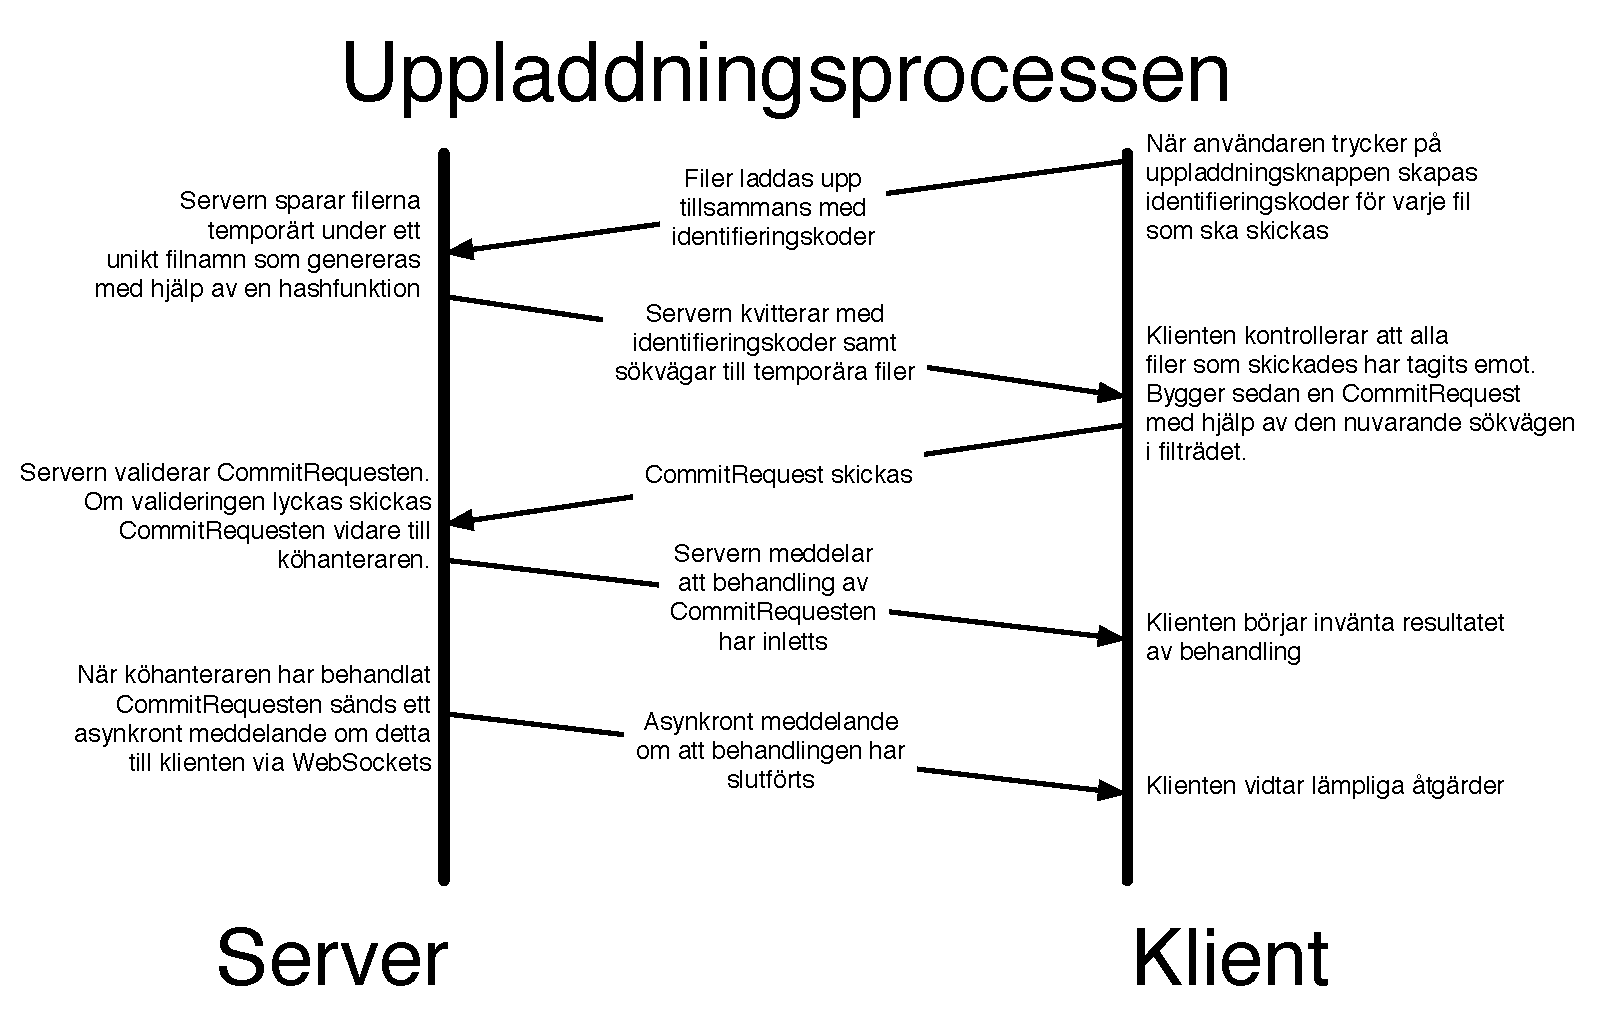
\includegraphics[width=15.0cm]{fig/misc/uppladdningsprocessen.pdf}             
  \caption[Uppladdningsprocessen]
  {Uppladdningsprocessen}
  \label{fig:uppladdning}
\end{figure}

\subsection{Inlämningens livscykel}

För att implementera inlämningsuppgiftens livscykel har tillståndshantering implementerats i LabHasGroup-entiteten. LabHasGroup representerar kopplingen mellan en laboration och en grupp.
Tillstånden beskrivs som följer, se även illustration \ref{fig:cyk}:

\begin{figure}
  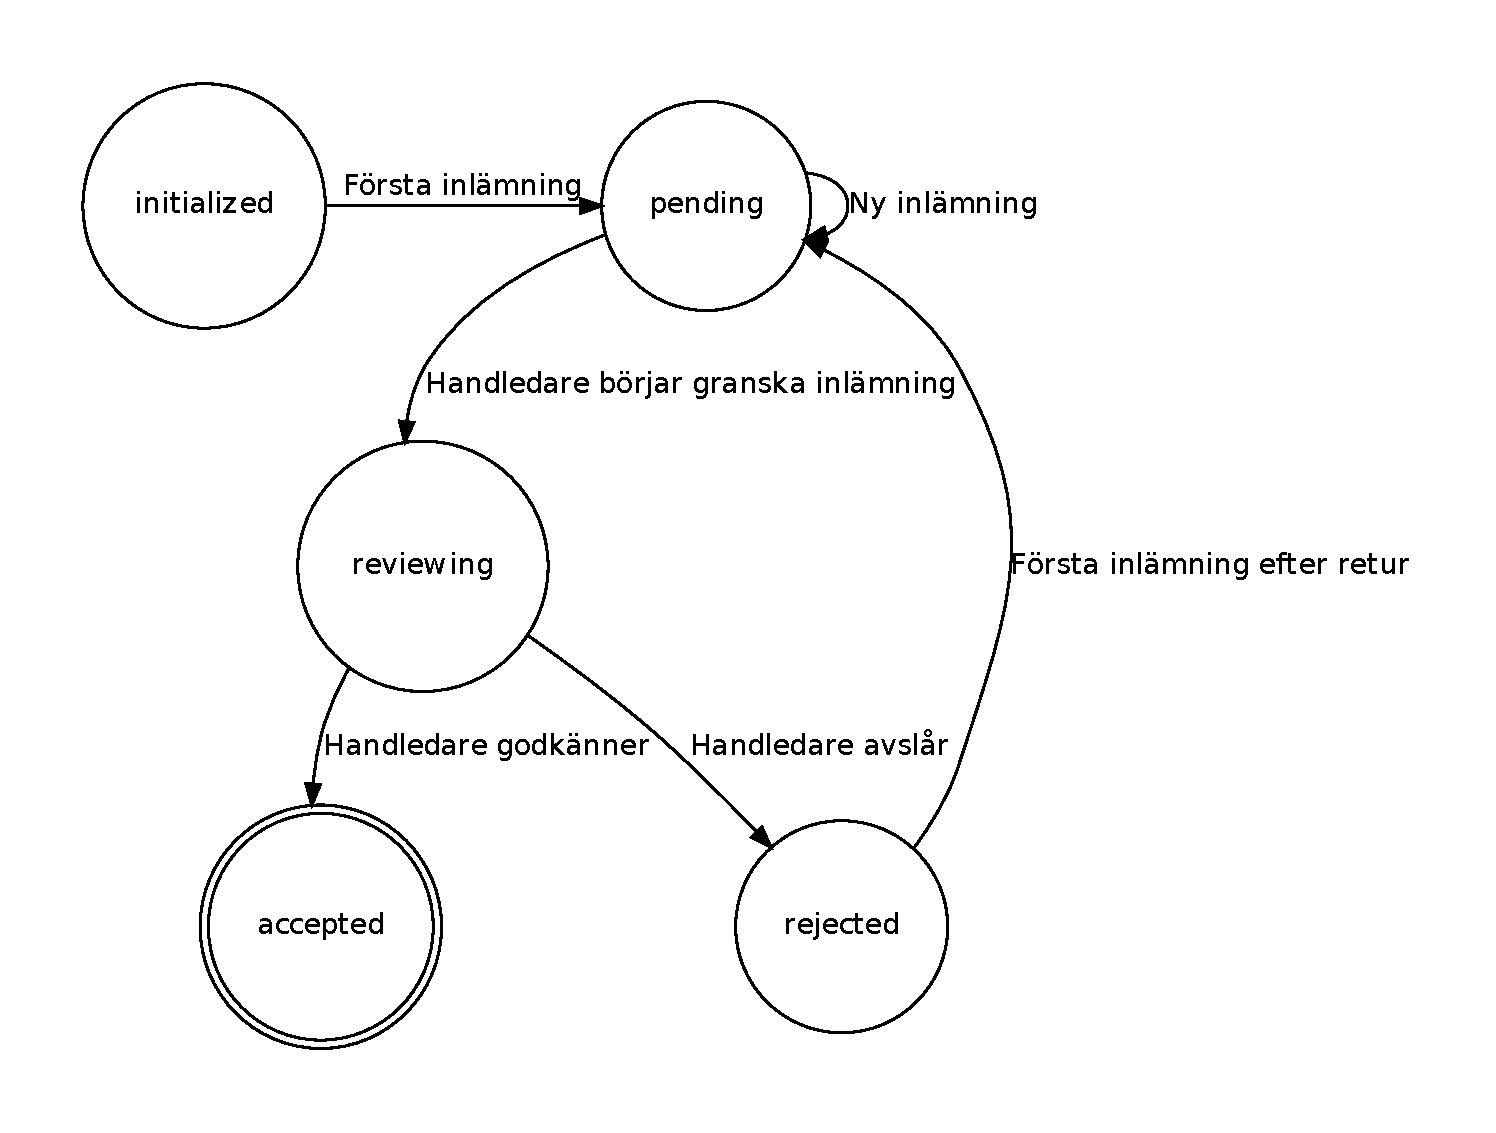
\includegraphics[width=15.0cm]{fig/labgroup/state-machine.pdf}             
  \caption[Inlämningsuppgiftens livscykel]
  {Inlämningens livscykel}
  \label{fig:cyk}
\end{figure}

\subsubsection{Initialized}

När en LabHasGroup skapas sätts objektet i tillståndet initialized. I detta tillstånd finns inga Submissions kopplade till entiteten och inlämning kan skapas fram tills dess att deadline har passerat.

\subsubsection{Pending}

När gruppen gör en inlämning skapas en Submission och LabHasGroup-entiteten övergår till tillståndet pending. Pending betyder att en inlämning är gjord, men att ingen handledare granskat laborationen.
Om en LabHasGroup befinner sig i pending kan dess senaste Submission uppdateras, fram tills dess att deadline har passerat, så att den pekar på ett nytt tillstånd i repositoriet.

\subsubsection{Reviewing}

Så snart en handledare har påbörjat granskningen en laboration övergår LabHasGroup-entiteten till tillståndet reviewing. I detta tillstånd är det inte möjligt att göra fler inlämningar.

\subsubsection{Rejected och Accepted}

Efter granskning kan handledaren godkänna eller förkasta inlämningen. Om inlämningen är godkänd går LabHasGroup-entiteten över i tillståndet accepted. Inga fler inlämningar tas emot. Om inlämningen förkastas går entiteten över i tillståndet rejected. I rejected-tillståndet är det möjligt att göra en ny inlämning, varpå tillståndet övergår i pending.

\section{CommitRequest: Ett API för manipulering av repositorier via webbklienten}
Webbgränssnittet utför operationer på Gitrepositorier genom att göra anrop till webbservern, som i sin tur förmedlar anropen till köhanteraren. Projektgruppen har valt att kalla dessa anrop för CommitRequest.
För anropen har projektgruppen definierat ett API. Samma dataformat används för att skicka vidare anropen från webbservern till köhanteraren.
Operationerna som stöds är:

\begin{itemize}
  
  \item add – Lägg till filer
  \item rm – Ta bort filer och mappar
  \item mkdir – Skapa en mapp
  \item mv – Flytta filer
  
\end{itemize}

Alla operationer kräver ett repositorie-id samt namnet på den branch som ska användas. Alla operationer stöder också att ett commit-meddelande skickas med anropet. Ett tomt commit-meddelande leder till att servern genererar ett automatiskt meddelande. Add och mv kräver en ursprungssökväg och en destinationssökväg. Rm och mkdir kräver bara sökvägar.
Se bilaga \ref{appendix:api} för en exakt specifikation.
\section{Hantering av roller}

För att användare ska ha tillgång till olika funktionalitet, beroende på vilken typ av användare de är har roller implementerats. Dessa roller är student, assistant, examiner och administrator. Funktionalitet för de olika rollerna befinner sig i en \emph{scope}, och en användare har bara tillgång till den funktionalitet som dess roll tillhandager. Om en användare är en adminstratör kan den skapa nya kurser, men en användare som är en student tillåts inte göra det.

\subsection{Rollernas påverkan på routes}
Användarfunktionaliteten befinner sig inom en \emph{scope} med roller. Detta ger upphov till estetiska, och intuitivt förstådda URL:er. Till exempel kan kurser visas upp för en student genom: |/student/courses|. Om studenten också är en Assistant, används en annan route för att visa relevant information för det sammahanget.

Sidor som till exempel visar en mall för redigering av User-information ska inte vara \emph{scopade}, eftersom de inte tillhör någon specifik roll-kontext.

\chapter{Resultat och diskussion}

\section{Resultat}
Resultatet av projektet är en mogen backend med ett vältestat modell-lager. Se kodtäckningsbilaga för mer information. Alla subsystem har implementerats, men med varierande grader av fullständighet.

Inlämning via Git är delvis funktionellt. Inlämning via webbgränssittet är i stort sett klart.

Webbgränssnittet för studenter är i stort sett klart. För handledare finns många viktiga funktioner implementerade.

Kommentarer har blivit implementerade för inlämningar.

Examinatorns och systemadministratörens gränssnitt har inte implementerats än.

\subsection{Implementerad funktionalitet}
Här presenteras funktionalitet som är implementerad när rapporten skrivs.
\subsubsection{Funktioner}
\begin{itemize}
	\item Webbgränssnitt
	\begin{itemize}
		\item Dashboard – visar viktig information om kurser, laborationer och inlämningar, implementerade för:
		\begin{itemize}
			\item Studenter
			\item Handledare
		\end{itemize}
		\item Bläddra i filsystem
		\item Rendering av källkod.
		\item Inlämningar
		\begin{itemize}
			\item Ladda upp en eller flera filer på samma gång
			\item Radera filer och mappar
			\item Skapa mappar
			\item Göra en inlämning, uppdatera en inlämning om rättningsprocessen inte har inleds
		\end{itemize}
		\item Grupphantering
		\begin{itemize}
			\item Skapa grupp i kurs
            \item Knyta grupp till laboration
            \item Knyta student till grupp med hjälp av inbjudningskod
		\end{itemize}
		\item Rättning
		\begin{itemize}
			\item Översikt över alla kurser med inlämningar som har kopplats till handledaren
            \item Lägga till handledares anteckning till Submission
            \item Lägga till inledande kommentar till Submission
            \item Godkänna eller underkänna en Submission
            \item Student och Assistent kan lägga till ytterligare kommentarer på en Submission
		\end{itemize}
	\end{itemize}
\end{itemize}

\subsubsection{Subsystem}

\begin{itemize}
  \item PostgreSQL-databas
  \item Ruby on Rails-applikation
  \item Faye – WebSocket-server
  \item Javascriptapplikationer
  \item Köhanterare med workers
  \item Grack – SmartHTTP-server
\end{itemize}

Planerad funktionalitet som inte implementerades

\begin{itemize}
  \item Validering av inlämningsuppgifter
  \item Noggrannare hantering av deadlines och hur de relaterar till inlämningar.
  \item Administration  
  \begin{itemize}
    \item Skapa och hantera kurser, inlämningsuppgifter och deadlines
    \item Delegering av rättigheter - implementerad i modellen men ej i gränssnittet
  \end{itemize}
  \item Visualisera diffar
  \item Grupphantering
  \begin{itemize}
    \item Hantering av situationer där gruppen vill splittras efter att arbetet har inletts.
  \end{itemize}
\end{itemize}
\input{include/diskussion/resonemang.tex}
\section{Rekommendationer}

Implementationen är inte klar. Nästa steg för systemet är därför att all kvarvarande planerad funktionalitet implementeras.

Ännu saknas implementation av valideringar, deadlines och administration - där deadlines och administration är kritiska funktionaliteter för att systemet skall kunna användas. 

\subsection{Administration}
Administration innefattar all form av hantering utav kurser och användare. Kurser behöver kunna skapas och rättigheter delegeras av någon administratör. Kursen i sin tur måste administreras av någon, förslagsvis examinatorn, som i sin tur måste kunna skapa, ta bort och redigera laborationer. Examinatorn borde även kunna registrera studenter på kursen och tillsätta handledare med speciella rättigheter. Slutligen skall implementationen av LADOK-kompatibla listor färdigställas.

\subsection{Deadlines}
Idag har varje laboration en deadline. Funktionaliteten för deadlines är dock inte implementerad. Det behövs restriktioner som stänger inlämningskanalerna efter att en deadline passerar. Därtill måste även logik för flera deadlines, samt hur man ska hantera utökade deadlines, implementeras. 

\subsection{Valideringar}
Enkla automatiska valideringar av formalia filnamn, filändelser och liknande är inte en nödvändig del av ett fungerande system, men är en potentiellt populär funktion som borde vara lätt att implementera.

\subsection{Diffar}

Möjligheten att snabbt se skillnader mellan två tillstånd i en inlämningsuppgift var en funktion som projektgruppen gärna hade implementerat.

\subsection{Testning}

Det är att föredra om ett testdrivet-utvecklingsätt används vid vidareutveckling då utvecklingssättet ger en mer verifierbar kodbas som enklare kan vidareutvecklas av andra utvecklare.

Testverktyget RSpec ger lättlästa tester, är lätt att lära sig och bör därför vara bland alternativen för test-ramverk inom framtida utveckling. För View-Controller tester rekommenderas Capybara.



\subsection{Kommentarer}
Förmågan att kommentera andra modeller utöver Submission har inte blivit implementerat. Det kan, till exempel, vara av intresse för studenter att kunna ställa frågor om en laboration via kommentarer. 

\subsection{Dokumentation}
För att göra systemet användbart för slutanvändarna måste en användarhandbok skrivas. 

För göra det möjligt för andra utvecklare att vidareutveckla systemet måste en mer gedigen dokumentation av kodbasen tas fram.



\chapter{Slutsatser}

Ruby on Rails är ett effektivt verktyg för att skapa stora webbapplikationer på kort tid och de som inte hade någon erfarenhet av Rails sen tidigare satte sig snabbt in i det.

Det finns många fördelar med testdriven-utveckling, buggar som skapar problem nu och längre fram i utvecklingen kan undvikas. Det är också lättare för en annan utvecklare att bygga på en tidigare feature om den har blivit grundligt testad. Nackdelen är att skriva tester tar en del av utvecklingstiden, men det är kandidatgruppens uppfattning att testning har större fördelar än nackdelar.

Vid utvecklingen av en sån här stor applikation är det viktigt att ha en noggrant genomtänkt databasmodell. Att göra större ändringar i en databas när utvecklingen av modell-lagret har nått långt är inte praktiskt då delar av modell-lagret kan behöva göras om.

Att bryta ner ett projekt i flertal funktionsorienterade subiterationer kan vara ett svårt tillvägagångssätt då många funktioner är beroende av varandra.

När en applikation ska anpassas till ett befintligt system krävs en detaljerad specifikation över vad som redan finns, vad som behöver tas bort och vad som behöver läggas till.

Parprogrammering visade sig vara ett bra sätt att ta sig an en uppgift, båda utvecklarnas kunskaper togs till vara och kunde flika in om de fick en idé. Genom att vara delaktiga lärde sig båda partnerna mer, då de kunde samarbeta och därmed arbeta fortare.


\renewcommand{\thechapter}{}
%\cleardoublepage
%\phantomsection
%\textsc{\Large Referenser}\\[0.5cm]
\chapter{Referenser}
\begin{flushleft}
\small

Atlassian (2012) Bamboo. \emph{Continuous Integration, Continuous Deployment and Build server Atlassian}. http://www.atlassian.com/software/bamboo/overview (2012-05-13)

Breit, L. (1998) Web server connectivity, performance. \emph{Unisys World}, vol. 19, nr. 7, ss. 8, 10.

Chacon, S. (2010) Smart HTTP Transport. \emph{Git}, http://git-scm.com/2010/03/04/smart-http.html (2012-05-10).

Chacon, S. (2009) \emph{Git on the Server - The Protocols. Pro Git}, Apress, New York.

Chalmers (2009) \emph{Akademisk hederlighet på Chalmers – Vilka är våra spelregler?}, https://document.chalmers.se/download?docid=986701354, (2012-05-13).

Chalmers (2012) Kurser på Chalmers. \emph{Sök i kursutbudet} . https://student.portal.chalmers.se/sv/chalmersstudier/minkursinformation/Sidor/SokKurs.aspx (2012-05-13).

Chalmers. (2008) \emph{Anonyma tentor}, https://student.portal.chalmers.se/sv/chalmersstudier/tentamen/Sidor/Anonyma-tentor.aspx, (2012-05-12).

ECMA (2011) Standard ECMA-262, \emph{ECMAScript Language Specification}, upplaga 5.1. Geneve: ECMA.

Gedell, T. (2006) \emph{Grading submissions - Review submission}, http://fire.cs.chalmers.se/doc/admin/grading-grade.html (2012-05-14).

Gedell, T. (2006) \emph{Upload File}, http://fire.cs.chalmers.se/doc/student/upload.html (2012-05-13).

Git (2012) \emph{git-clone(1) Manual Page}. http://git-scm.com/docs/git-clone (2012-05-13).

Gitorious (2007) About Gitorious. \emph{ About - Gitorious}. http://www.gitorious.org/about (2012-05-07).

GNU (2007) GNU Affero General License. \emph{GNU Affero General Public License - GNU Project - Free Software Foundation (FSF)}. http://www.gnu.org/licenses/agpl-3.0.html,(2012-05-06).

GNU (2012) What is Copyleft?. \emph{What is Copyleft? - GNU Project - Free Software Foundation (FSF)}. http://www.gnu.org/copyleft/,(2012-05-06).

Internet Engineering Task Force (2011) \emph{RFC 2616 Hypertext Transfer Protocol -- HTTP/1.1}, Fielding, et al.: IETF.

Internet Engineering Task Force (2011) \emph{RFC 6455 The WebSocket Protocol}, Fette, I., Melnikov, A.: IETF.

Jenkins (2012) \emph{Meet Jenkins}, https://wiki.jenkins-ci.org/display/JENKINS/Meet+Jenkins, (2012-05-14).

Launchpad (2010) LaunchpadLicense. \emph{LaunchpadLicense - Launchpad Development}. https://dev.launchpad.net/LaunchpadLicense, (2012-05-14).

Launchpad (2009) Launchpad is now open source. \emph{Launchpad Blog} http://blog.launchpad.net/general/launchpad-is-now-open-source (2012-02-09).

Lilleaas, A. (2010) Work on Rails 3 upgrade has started. \emph{Work on Rails 3 upgrade has started - Google Groups}. https://groups.google.com/group/gitorious/browse\_thread/thread/16c4a60d760c0c07/ca246703db19f3ce?pli=1, (2012-05-14).

Mesbah, A., van Deursen, A. (2008) A component- and push-based architectural style for ajax applications. \emph{Journal of Systems and Software}, vol. 81, nr. 12, ss. 2194-2209.

Mlodgenski, J. (2010) PostgreSQL vs. MySQL: How to Select the Right Open-Source Database. \emph{eWeek}. 2010-10-21.  http://www.eweek.com/c/a/Linux-and-Open-Source/PostgreSQL-vs-MySQL-How-to-Select-the-Right-OpenSource-Database/ (2012-05-11).

O'Sullivan, B. (2009) Making Sense of Revision-Control Systems. \emph{Communications of the ACM}, vol. 52, nr. 9, ss. 56-62, Doi:10.1145/1562164.1562183.

Preston-Werner, T. (2011) \emph{Ten Lessons from GitHub's First Year}. http://tom.preston-werner.com/2011/03/29/ten-lessons-from-githubs-first-year.html (2012-05-13).

Rails webblog (2008) This Week in Edge Rails. \emph{Riding Rails: This Week in Edge Rails}. http://weblog.rubyonrails.org/2008/11/28/this-week-in-edge-rails/, (2012-05-14).

Rarick, K. (2007) \emph{About - beanstalkd}, http://kr.github.com/beanstalkd/ (2012-05-14).

Rubyforge (2012) Rack::Builder. \emph{Class: Rack::Builder}. http://rack.rubyforge.org/doc/classes/Rack/Builder.html (2012-05-13).

TIOBE Software (2012) TIOBE Programming Community Index for May 2012. \emph{TIOBE Software: Tiobe Index}. http://www.tiobe.com/index.php/content/paperinfo/tpci/index.html (2012-05-13).

URKUND. (2012), Integrera URKUND i organisationens lärplattform. \emph{Urkund}. http://www.urkund.se/SE/uoh\_integration.asp, (2012-05-13).

Vaughan-Nichols, S. (2007), Last of the GPL Licenses Goes to Version 3; The Free Software Foundation has released the GNU Affero General Public License Version 3, the open-source over-a-network license, to general use. (Linux-Watch), \emph{eWeek} (2012-05-06).

Wang, T.J et al (2010), Accounting For The Benefits Of Database Normalization. \emph{American Journal of Business Education}, vol 3, nr 1, ss. 41-52.

\normalsize
\end{flushleft}


\newpage
\clearpage


\setspecialhdr

\newpage

% Appendices
\appendix
\setdefaulthdr
\chapter{CommitRequest-API}

\pagebreak

\begin{lstlisting}[language=Ruby, showstringspaces=false]
  {
    repository: 123,
    command: "mkdir"
    branch: "master",
    commit_message: "A message",
    path: "path/to/dir"
  }
  {
    repository: 123,
    command: "add"
    branch: "master",
    commit_message: "A message",
    files: [{
      from: "path/to/dir/and/file.file",
      to: "path/to/dir/and/file.file"
    }]
  }
  {
    repository: 123,
    command: "move"
    branch: "master",
    commit_message: "A message",
    records: [{
      from: "path/to/file.txt",
      to: "path/to/new_file.txt"
    }]
  }
  {
    repository: 123,
    command: "remove"
    branch: "master",
    commit_message: "A message",
    records: [
      "path/to/file1.txt", 
      "path/to/file2.txt"
    ]
  }
\end{lstlisting}

\end{document}
